% */ vim: set tw=150: */
\documentclass[11pt,a4paper]{article}
\pdfoutput=1

\usepackage{amsmath}
\usepackage[T1]{fontenc}

\usepackage{jheppub}
\usepackage{psfrag}
\usepackage{slashed}
\usepackage{cancel}
\usepackage{lscape}
\usepackage{caption}
\usepackage{array}
\usepackage{graphicx}
\usepackage{subcaption}
\usepackage{multirow}
\usepackage{tabularx}
\usepackage{makecell}
\usepackage[utf8]{inputenc}
\usepackage{amsmath}
\usepackage{amssymb}
\usepackage{relsize}
\usepackage{color}
\usepackage{slashed}
\usepackage{mathtools}
\usepackage{comment}
\usepackage{scalefnt}
\usepackage{siunitx}[=v2]
\sisetup{
    round-mode = off,
    round-precision = 4,
    scientific-notation = false,
    fixed-exponent = 0,
    group-digits = true,
    group-separator = {\,},
}

%{{{ macros

\renewcommand{\arraystretch}{1.3}

\definecolor{mypink}{RGB}{219, 48, 122}
\definecolor{mygreen}{rgb}{0,0.7,0}
\definecolor{raspberry}{rgb}{0.53,0.15,0.34}
\def\SB#1{\textcolor{mygreen}{{\bf\tt [SB: #1]}}}
\def\SZ#1{\textcolor{raspberry}{{\bf\tt [SZ: #1]}}}

%%% spinor products %%%

\def\zz{\boldsymbol{Z}}
\def\mi{\mathrm{MI}}
\def\cF{\mathcal{F}}
\def\cP{\mathcal{P}}
\def\cC{\mathcal{C}}
\def\cA{\mathcal{A}}
\def\cN{\mathcal{N}}
\def\cO{\mathcal{O}}
\def\cD{\mathcal{D}}
\def\cQ{\mathcal{Q}}
\def\cJ{\mathcal{J}}
\def\cI{\mathcal{I}}
\def\cT{\mathcal{T}}
\def\nn{\nonumber \\ }

\def\la{\langle}
\def\ra{\rangle}
\def\spA#1#2{\la#1#2\ra}
\def\spB#1#2{[#1#2]}
\def\spAB#1#2#3{\la#1|#2|#3]}
\def\spBA#1#2#3{[#1|#2|#3\ra}
\def\spAA#1#2#3{\la#1|#2|#3\ra}
\def\spBB#1#2#3{[#1|#2|#3]}
\def\spab#1#2{\la#1|#2]}
\def\spaa#1#2#3#4{\la#1|#2|#3|#4\ra}
\def\spbb#1#2#3#4{[#1|#2|#3|#4]}
\def\wh#1{\widehat#1}
\DeclareMathOperator{\tr}{\rm tr}
\def\trm{\tr_-}
\def\trp{\tr_+}
\def\MP#1#2{(#1\cdot#2)}
\def\trfive{\tr_5}
\def\spAXB#1#2#3#4#5{\la#1|#2|#3|#4|#5]}

\def\bra#1{\langle #1|}
\def\ket#1{|#1 \rangle}
\def\sqbra#1{[#1|}
\def\sqket#1{|#1]}
\def\braket#1{\langle #1 \rangle}

\def\eps{\epsilon}
\def\fl#1{#1^\flat}
\def\tl#1{\tilde{#1}}
\def\wh{\widehat}
\def\tC{\tilde{C}}
\def\qb{{\bar{q}}}
\def\sb{\bar{s}}
\def\Sb{\bar{S}}
\def\lb{\bar{\ell}}
\def\tb{{\bar{t}}}
\def\ttgg{\bar{t}tgg}
\def\mren{\mathrm{mren}}
\def\ren{\mathrm{ren}}
\def\mct{\mathrm{mct}}
\def\ceps{C_\eps}
\def\as{\alpha_s}
\def\dk#1{\frac{d^d k_{#1}}{i\pi^{d/2}e^{-\eps \gamma_E}}}

\def\e{\epsilon}
\def\tT{\tilde{T}}
\def\coll#1#2{\overset{#1||#2}{\to}}
\def\inf{{\rm Inf}}
\def\gg#1{\gamma_{#1}}
\def\XX{\chi}

\def\cv#1#2{\AB{#1}{\gamma^\mu}{#2}}
\def\cvS#1#2#3{\AB{#1}{#2}{#3}}

\def\MHVb{$\overline{\rm MHV}$}
\def\boxX{$\xcancel{\rm\bf box}$}

\def\fl#1{{#1^{\flat}}}
\def\flm#1{{#1^{\flat,\mu}}}
\def\kf#1{{\fl{K_{#1}}}}
\def\kfm#1{{\flm{K_{#1}}}}

\def\ulim#1{\underset{#1}{\lim}}

\def\fbox#1{F^{(#1)}_{\mathrm{box}}}
\def\lh{\hat{L}}
\def\li#1{\mathrm{Li}_{#1}}

\def\finr{{\mathcal{F}}}
\def\pole{{\mathcal{P}}}
\def\cusp{{\mathrm{cusp}}}

\newcommand{\njet}{\texttt{NJet}}
\newcommand{\pentagonfunctions}{\texttt{PentagonFunctions++}}
\newcommand{\finiteflow}{\texttt{FiniteFlow}}
\newcommand{\qd}{\texttt{QD}}
\newcommand{\eigen}{\texttt{Eigen}}
\newcommand{\nnlojet}{\texttt{NNLOJET}}
\newcommand{\mathematica}{\texttt{Mathematica}}
\newcommand{\form}{\texttt{FORM}}
\newcommand{\qgraf}{\texttt{QGRAF}}
\newcommand{\spinney}{\texttt{Spinney}}
\newcommand{\cpp}{\texttt{C++}}
\DeclareMathOperator{\Tr}{Tr}

%%Christian's command
\newcommand{\eqcite}[1]{(\ref{#1})}
\newcommand{\dd}{\mathop{}\!\mathrm{d}}

\newcommand{\fp}{\texttt{f64}}
\newcommand{\fpp}{\texttt{f128}}
\newcommand{\fppp}{\texttt{f256}}

%%%% typesetting equations %%%%
\def\s#1{s_{#1}}
\def\d#1#2{#1\cdot #2}
\def\p#1{#1}
\def\pp#1{p_{#1}}
\def\f#1{#1^\flat}
\def\n#1{\eta_{#1}}

\def\Adcc{B_n^{(1)}}

\def\usepic#1#2{\parbox{#1}{\includegraphics[width=#1]{#2}}}
\def\usepix#1#2#3#4#5#6{\parbox{#1}{\includegraphics[width=#1,trim= #3 #4 #5 #6,clip=true]{#2}}}

\def\hpl11{{\mathrm{HPL}}_{1,1}}

\newcolumntype{C}[1]{>{\hsize=#1\hsize\centering\arraybackslash}X}%

\newcolumntype{Z}{r<{\hspace{3mm}}}
\newcommand\mc[2]{\multicolumn{1}{>{\centering}p{#2}}{#1}} % handy shortcut macro
% }}}

%%\allowdisplaybreaks

\newcommand{\MSbar}{\ensuremath{\overline{\text{MS}}}}
\newcommand{\fonll}{FONLL}
\newcommand{\nlonnllpart}{NLO+NNLL\textsubscript{part}+$y_by_t$}
\newcommand{\nnnres}{$\text{N}^3\text{LL'}+\text{aN}^3\text{LO}$}

\providecommand{\href}[2]{#2}

\newcommand{\incl}{{\tt inclusive}}
\newcommand{\fidYR}{{\tt fiducial-YR}}
\newcommand{\fidATLAS}{{\tt fiducial-ATLAS}}

\newcommand{\stepone}{{Step\,I}}
\newcommand{\steptwo}{{Step\,II}}
\newcommand{\stepthree}{{Step\,III}}

\newcommand\tS{\tilde{S}}
\newcommand\F{${\textrm F}$}
\newcommand\FJ{${\textrm FJ}$}
\newcommand\FJJ{${\textrm FJJ}$}
\newcommand\PhiBorn{\Phi_{\scriptscriptstyle \textrm B}}
\newcommand\PhiReal{\Phi_{\scriptscriptstyle \textrm R}}
%\newcommand\PhiB{\Phi_{\scriptscriptstyle \textrm H}}
\newcommand\PhiB{\Phi_{\scriptscriptstyle \textrm F}}
\newcommand\PhiBres{\Phi_{\scriptscriptstyle \textrm F,res}}

\newcommand{\flav}{\ell}
\newcommand{\flavBorn}{\flav_{\scriptscriptstyle \textrm B}}
\newcommand{\fullflavBorn}{\hat \flav_{\scriptscriptstyle \textrm B}}
\newcommand{\flavprimeBorn}{\flav'_{\scriptscriptstyle \textrm B}}
\newcommand{\fullflavprimeBorn}{\hat \flav'_{\scriptscriptstyle \textrm B}}
\newcommand{\flavB}{\flav_{\scriptscriptstyle \textrm F}}
\newcommand{\fullflavB}{\hat \flav_{\scriptscriptstyle \textrm F}}
\newcommand{\flavBJ}{\flav_{\scriptscriptstyle \textrm FJ}}
\newcommand{\fullflavBJ}{\hat \flav_{\scriptscriptstyle \textrm FJ}}
\newcommand{\flavBJJ}{\flav_{\scriptscriptstyle \textrm FJJ}}
\newcommand{\fullflavBJJ}{\hat \flav_{\scriptscriptstyle \textrm FJJ}}
\newcommand{\projflav}{\flavB\leftarrow\flavBJ}
\newcommand{\CF}{C_{\mathrm{F}}}
\newcommand{\CA}{C_{\mathrm{A}}}
\newcommand{\NC}{N_{\mathrm{c}}}
\newcommand{\nf}{N_f}
\newcommand{\TF}{T_{\mathrm{F}}}

\newcommand{\flavZg}{\flav_{\scriptscriptstyle Z\gamma}}
\newcommand{\fullflavZg}{\hat \flav_{\scriptscriptstyle Z\gamma}}
\newcommand{\flavZgJ}{\flav_{\scriptscriptstyle Z\gamma {\textrm J}}}
\newcommand{\fullflavZgJ}{\hat \flav_{\scriptscriptstyle Z\gamma {\textrm J}}}
\newcommand{\flavZgJJ}{\flav_{\scriptscriptstyle Z\gamma {\textrm J}}}
\newcommand{\fullflavZgJJ}{\hat \flav_{\scriptscriptstyle Z\gamma {\textrm J}}}
\newcommand{\projflavZg}{\flavZg\leftarrow\flavZgJ}

%\newcommand\PhiBJ{\Phi_{\scriptscriptstyle \textrm HJ}}
\newcommand\PhiBJ{\Phi_{\scriptscriptstyle \textrm FJ}}
\newcommand\ZJ{Z\gamma J}
\newcommand\PhiZJ{\Phi_{\scriptscriptstyle \textrm Z\gamma J}}
\newcommand\PhiBJbar{{\bar \Phi}'_{\scriptscriptstyle \textrm FJ}}
\newcommand\PhiBJJ{\Phi_{\scriptscriptstyle \textrm FJJ}}
\newcommand\PhiZJJ{\Phi_{\scriptscriptstyle \textrm Z\gamma JJ}}
\newcommand\PhiZgam{\Phi_{\scriptscriptstyle \textrm Z\gamma}}
\newcommand{\Fcorr}{F^{\tmop{corr}}_\ell}
\newcommand{\order}[1]{{\cal O}\left(#1\right)}
\newcommand{\aew}{\alpha_{\text{\scalefont{0.77}EW}}} 
\newcommand{\aw}{\alpha_w}
\newcommand{\asCMW}{\alpha_s^{\textrm †CMW}}
%\newcommand{\cO}[1]{{\cal O}\left(#1\right)}
\newcommand{\NNLL}{\text{NNLL}}
\newcommand{\eff}{\epsilon}
\newcommand{\ee}{\ell^+\ell^-}
\newcommand{\kt}[1]{k_{\scaleto{\textrm T}{4pt},#1}}
\newcommand{\veckt}[1]{\vec{k}_{\scaleto{\textrm T}{4pt},#1}}
%\newcommand{\dk}[1]{\langle \mathd k_{#1}\rangle}
\newcommand{\fullF}{\mathcal{F}}
\newcommand{\FNLL}{\mathcal{F}_{\textrm NLL}}
\newcommand{\FNNLL}{\mathcal{F}_{\textrm NNLL}}
\newcommand{\ie}{i.e.\,}
\newcommand{\css}{\text{\scriptsize CSS}}
\newcommand{\zi}{z_i^{(\ell_i)}}
\newcommand{\pt}{p_{\text{\relscale{0.77}T}}}
\newcommand{\GZ}{{\Gamma_Z}}
\newcommand{\GW}{{\Gamma_W}}
\newcommand{\thW}{{\theta_W}}
\newcommand{\mtop}{{m_{\text{\relscale{0.77}top}}}}
\newcommand{\qt}{{q_{\text{\relscale{0.77}T}}}}
\newcommand{\ptarg}[1]{{p_{\text{\relscale{0.77}T,$#1$}}}}
\newcommand{\marg}[1]{{m_{\text{\relscale{0.77}$#1$}}}}
\newcommand{\ptg}{p_{\text{\relscale{0.77}T,$\gamma$}}}
\newcommand{\ptgcut}{{p_{\text{\relscale{0.77}T,$\gamma$}}^{\textrm cut}}}
\newcommand{\ptjcut}{{p_{\text{\relscale{0.77}T,$j$}}^{\textrm cut}}}

%%newdef
\newcommand{\ptjmin}{\bar{p}_{\text{\relscale{0.77}T,$j$}}}
\newcommand{\ptgmin}{\bar{p}_{\text{\relscale{0.77}T,$\gamma$}}}
\newcommand{\ptgone}{p_{\text{\relscale{0.77}T,$\gamma_1$}}}
\newcommand{\ptgtwo}{p_{\text{\relscale{0.77}T,$\gamma_2$}}}
\newcommand{\ptgthree}{p_{\text{\relscale{0.77}T,$\gamma_3$}}}

\newcommand{\ptr}{{p_{\text{\relscale{0.77}T}}}^{\text{\relscale{0.9}r}}}
\newcommand{\ptrad}{{p_{\text{\relscale{0.77}T,rad}}}}
\newcommand{\pth}{{p_{\text{\relscale{0.77}T,$H$}}}}
\newcommand{\ptz}{{p_{\text{\relscale{0.77}T,$Z$}}}}
\newcommand{\ptw}{{p_{\text{\relscale{0.77}T,$W$}}}}
\newcommand{\ptnu}{{p_{\text{\relscale{0.77}T,$\nu$}}}}
\newcommand{\mtwz}{{m_{\text{\relscale{0.77}T,$WZ$}}}}
\newcommand{\dphiwz}{{\Delta\phi_{\text{\relscale{0.77}$WZ$}}}}
\newcommand{\dyZlW}{{|y_{\text{\relscale{0.77}$Z$}}-y_{\text{\relscale{0.77}$
\ell_W$}}|}}
\newcommand{\ptww}{{p_{\text{\relscale{0.77}T,$WW$}}}}
\newcommand{\ptwp}{{p_{\text{\relscale{0.77}T,$W^+$}}}}
\newcommand{\ptwm}{{p_{\text{\relscale{0.77}T,$W^-$}}}}
\newcommand{\mtww}{{m_{\text{\relscale{0.77}T,$WW$}}}}
\newcommand{\mtwwexp}{{m_{\text{\relscale{0.77}T,$WW$}}^{\textrm exp}}}
\newcommand{\ptllg}{{p_{\text{\relscale{0.77}T,}\ell\ell\gamma}}}
\newcommand{\ptzg}{\ptllg}
\newcommand{\ptll}{{p_{\text{\relscale{0.77}T,$e^+e^-$}}}}
\newcommand{\ptlnu}{{p_{\text{\relscale{0.77}T,$\mu\nu_\mu$}}}}
\newcommand{\ptj}{p_{\text{\relscale{0.77}T,$j$}}}
\newcommand{\ptjone}{{p_{\text{\relscale{0.77}T,$j_1$}}}}
\newcommand{\ptjoneveto}{{p_{\text{\relscale{0.77}T,$j_1$}}^{\textrm veto}}}
\newcommand{\ptjtwo}{{p_{\text{\relscale{0.77}T,$j_2$}}}}
\newcommand{\ptlm}{{p_{\text{\relscale{0.77}T,$\ell^-$}}}}
\newcommand{\ptl}{{p_{\text{\relscale{0.77}T,$\ell$}}}}
\newcommand{\ptlone}{{p_{\text{\relscale{0.77}T,$\ell_1$}}}}
\newcommand{\ptltwo}{{p_{\text{\relscale{0.77}T,$\ell_2$}}}}
\newcommand{\ptmiss}{{p_{\text{\relscale{0.77}T,miss}}}}
\newcommand{\ptmissrel}{{p_{\text{\relscale{0.77}T,miss,rel}}}}
\newcommand{\yh}{{y_{\text{\relscale{0.77}H}}}}
\newcommand{\yz}{{y_{\text{\relscale{0.77}Z}}}}
\newcommand{\ywp}{{y_{\text{\relscale{0.77}$W^+$}}}}
\newcommand{\yl}{{y_{\text{\relscale{0.77}$\ell$}}}}
\newcommand{\ylone}{{y_{\text{\relscale{0.77}$\ell_1$}}}}
\newcommand{\dphill}{{\Delta\phi_{\text{\relscale{0.77}$\ell_1\ell_2$}}}}
\newcommand{\yww}{{y_{\text{\relscale{0.77}$WW$}}}}
\newcommand{\yjone}{{y_{\text{\relscale{0.77}$j_1$}}}}
\newcommand{\dyww}{{\Delta y_{\text{\relscale{0.77}$W^-,W^+$}}}}
\newcommand{\mh}{{m_{\text{\relscale{0.77}H}}}}
\newcommand{\mz}{{m_{\text{\relscale{0.77}Z}}}}
\newcommand{\mw}{{m_{\text{\relscale{0.77}W}}}}
\newcommand{\mww}{{m_{\text{\relscale{0.77}WW}}}}
\newcommand{\mwsq}{{m^2_{\text{\relscale{0.77}W}}}}
\newcommand{\mt}{{m_{\text{\relscale{0.77}t}}}}
\newcommand{\mT}{{m_{\text{\relscale{0.77}T}}}}
\newcommand{\mgj}{{m_{\text{\relscale{0.77}$\gamma j_1$}}}}
\newcommand{\mllg}{{m_{\text{\relscale{0.77}$\ell\ell\gamma$}}}}
\newcommand{\mlnu}{{m_{\text{\relscale{0.77}$\mu\nu_\mu$}}}}
\newcommand{\etal}{{\eta_{\text{\relscale{0.77}$\ell$}}}}
\newcommand{\etallg}{{\eta_{\text{\relscale{0.77}$\ell\ell\gamma$}}}}
\newcommand{\etalone}{{\eta_{\text{\relscale{0.77}$\ell_1$}}}}
\newcommand{\etaltwo}{{\eta_{\text{\relscale{0.77}$\ell_2$}}}}
\newcommand{\etag}{{\eta_{\text{\relscale{0.77}$\gamma$}}}}
\newcommand{\etaj}{{\eta_{\text{\relscale{0.77}j}}}}
\newcommand{\etah}{{\eta_{\text{\relscale{0.77}H}}}}
\newcommand{\detallgj}{{\Delta\eta_{\text{\relscale{0.77}$\ell\ell\gamma, j_1$}}}}
\newcommand{\dphillg}{{\Delta\phi_{\text{\relscale{0.77}$\ell\ell,\gamma$}}}}
\newcommand{\drlg}{{\Delta R_{\text{\relscale{0.77}$\ell \gamma$}}}}
\newcommand{\drgjone}{{\Delta R_{\text{\relscale{0.77}$\gamma j_1$}}}}
\newcommand{\drgjtwo}{{\Delta R_{\text{\relscale{0.77}$\gamma j_2$}}}}
\newcommand{\drej}{{\Delta R_{\text{\relscale{0.77}$e j$}}}}

%new def
\newcommand{\rjg}{R_{\text{\relscale{0.77}$j \gamma$}}}
\newcommand{\rjgone}{R_{\text{\relscale{0.77}$j \gamma_1$}}}
\newcommand{\rjgtwo}{R_{\text{\relscale{0.77}$j \gamma_2$}}}
\newcommand{\rjgthree}{R_{\text{\relscale{0.77}$j \gamma_3$}}}
\newcommand{\rjgmin}{\bar{R}_{\text{\relscale{0.77}$j \gamma$}}}
\newcommand{\rjonegone}{R_{\text{\relscale{0.77}$j_1 \gamma_1$}}}
\newcommand{\rjonegtwo}{R_{\text{\relscale{0.77}$j_1 \gamma_2$}}}
\newcommand{\rjonegthree}{R_{\text{\relscale{0.77}$j_1 \gamma_3$}}}
\newcommand{\rjtwogone}{R_{\text{\relscale{0.77}$j_2 \gamma_1$}}}
\newcommand{\rjtwogtwo}{R_{\text{\relscale{0.77}$j_2 \gamma_2$}}}
\newcommand{\rjtwogthree}{R_{\text{\relscale{0.77}$j_2 \gamma_3$}}}


\newcommand{\lw}{\ensuremath{\mu}}
\newcommand{\lpw}{\ensuremath{\ell^+_{\text{\relscale{0.77}W}}}}
\newcommand{\lmw}{\ensuremath{\ell^-_{\text{\relscale{0.77}W}}}}
\newcommand{\lpmw}{\ensuremath{\ell^{\pm}_{\text{\relscale{0.77}W}}}}

\newcommand{\lz}{\ensuremath{e}}
\newcommand{\lpz}{\ensuremath{e^+}}
\newcommand{\lmz}{\ensuremath{e^-}}
\newcommand{\lpmz}{\ensuremath{e^{\pm}_{\text{\relscale{0.77}}}}}
\newcommand{\lzlead}{\ensuremath{e_{\text{\relscale{0.77}Z,1}}}}
\newcommand{\lzsubl}{\ensuremath{e_{\text{\relscale{0.77}Z,2}}}}

\newcommand{\ptlz}{\ensuremath{p_{\text{\relscale{0.77}T,\lz}}}}
\newcommand{\ptlw}{\ensuremath{p_{\text{\relscale{0.77}T,\lw}}}}
\newcommand{\ptlzlead}{\ensuremath{p_{\text{\relscale{0.77}T,\lzlead}}}}
\newcommand{\ptlzsubl}{\ensuremath{p_{\text{\relscale{0.77}T,\lzsubl}}}}

\newcommand{\mlll}{\ensuremath{m_{\text{\relscale{0.77}$3\ell$}}}}
\newcommand{\mwz}{\ensuremath{m_{\text{\relscale{0.77}WZ}}}}
\newcommand{\mtw}{\ensuremath{m_{\text{\relscale{0.77}T,W}}}}
\newcommand{\ptwz}{\ensuremath{p_{\text{\relscale{0.77}T,WZ}}}}
\newcommand{\ptlp}{\ensuremath{p_{\text{\relscale{0.77}T,\ell'}}}}
\newcommand{\dRll}{\ensuremath{\Delta R_{\text{\relscale{0.77}$\ell\ell$}}}}
\newcommand{\dRllp}{\ensuremath{\Delta R_{\text{\relscale{0.77}$\ell\ell'$}}}}
\newcommand{\etalp}{\ensuremath{\eta_{\text{\relscale{0.77}$\ell'$}}}}

\newcommand{\qcdfull}{\ensuremath{\text{NNLO}_{\textrm QCD}^{{\textrm (QCD,QED)}_{\textrm PS}}}}
\newcommand{\qcdqcd}{\ensuremath{\text{NNLO}_{\textrm QCD}^{{\textrm (QCD)}_{\textrm PS}}}}

\newcommand{\addfull}{\ensuremath{\text{NNLO}_{\textrm QCD}^{\textrm (QCD,QED)_{\textrm PS}} + \delta{\textrm NLO}_{\textrm EW}^{\textrm (QCD,QED)_{\textrm PS}}}}
\newcommand{\addqcdfull}{\ensuremath{\text{NNLO}_{\textrm QCD}^{\textrm (QCD,QED)_{\textrm PS}} + \delta{\textrm NLO}_{\textrm EW}^{\textrm (QED)_{\textrm PS}}}}
\newcommand{\addqedfull}{\ensuremath{\text{NLO}_{\textrm EW}^{\textrm (QCD,QED)_{\textrm PS}} + \delta{\textrm NNLO}_{\textrm QCD}^{\textrm (QCD)_{\textrm PS}}}}

\newcommand{\multfull}{\ensuremath{\text{NNLO}_{\textrm QCD}^{\textrm (QCD,QED)_{\textrm PS}} \times \text{K-NLO}_{\textrm EW}^{\textrm (QCD,QED)_{\textrm PS}}}}
\newcommand{\multqcdfull}{\ensuremath{\text{NNLO}_{\textrm QCD}^{\textrm (QCD,QED)_{\textrm PS}} \times \text{K-NLO}_{\textrm EW}^{\textrm (QED)_{\textrm PS}}}}
\newcommand{\multqedfull}{\ensuremath{\text{NLO}_{\textrm EW}^{\textrm (QCD,QED)_{\textrm PS}} \times \text{K-NNLO}_{\textrm QCD}^{\textrm (QCD)_{\textrm PS}}}}

\newcommand{\multmatrix}{\ensuremath{\text{NNLO}_{\textrm QCD}^{\textrm (QCD)_{\textrm PS}} \times \text{K-NLO}_{\textrm EW}^{\text{\Matrix{}}}}}
\newcommand{\QCDpEW}{\ensuremath{ \text{NNLO}_{\textrm QCD+EW}^{\textrm (QCD, QED)_{\textrm PS}}}} 
\newcommand{\QCDtEW}{\ensuremath{ \text{NNLO}_{\textrm QCDxEW}^{\textrm (QCD, QED)_{\textrm PS}}}} 
\newcommand{\QCDtEWfo}{\ensuremath{ \text{NNLO}_{\textrm QCD}^{\textrm (QCD)_{\textrm PS}} \times \text{K-NLO}_{\textrm EW}^{\textrm (f.o.)}}} 



\newcommand{\drlj}{{\Delta R_{\text{\relscale{0.77}$\ell,j$}}}}
\newcommand{\drgj}{{\Delta R_{\text{\relscale{0.77}$\gamma j$}}}}
\newcommand{\drgjo}{{\Delta R_{\text{\relscale{0.77}$\gamma j_1$}}}}
\newcommand{\drgjt}{{\Delta R_{\text{\relscale{0.77}$\gamma j_2$}}}}
\newcommand{\fcl}{{E_{\text{\relscale{0.77}T}}^{\text{\relscale{0.77}cone$0.2$}}/p_{\text{\relscale{0.77}T},\gamma}}}
\newcommand{\muF}{{\mu_{\text{\relscale{0.77}F}}}}
\newcommand{\muR}{{\mu_{\text{\relscale{0.77}R}}}}
\newcommand{\muB}{{\mu_{\text{\relscale{0.77}B}}}}
\newcommand{\muFtwo}{{\mu^2_{\text{\relscale{0.77}F}}}}
\newcommand{\muRtwo}{{\mu^2_{\text{\relscale{0.77}R}}}}
\newcommand{\muFc}{{\mu_{\text{\relscale{0.77}F},0}}}
\newcommand{\muRc}{{\mu_{\text{\relscale{0.77}R},0}}}
\newcommand{\muRy}{{\mu_{\text{\relscale{0.77}R}}^{(0),y}}}
\newcommand{\muRb}{{\mu_{\text{\relscale{0.77}R}}^{(0),\alpha}}}
\newcommand{\KF}{K_{\text{\relscale{0.77}F}}}
\newcommand{\KR}{K_{\text{\relscale{0.77}R}}}
\newcommand{\KRy}{{K^y_{\text{\relscale{0.77}R}}}}
\newcommand{\KQ}{{K_{\text{\relscale{0.77}Q}}}}
\newcommand{\Q}{{Q_{\text{\relscale{0.77}$0$}}}}
\newcommand{\Qc}{{Q_{\text{\relscale{0.77}res},0}}}

\newcommand{\noun}[1]{{\scshape #1}}
\newcommand{\MADGRAPH}{\noun{MadGraph v4}}
\newcommand{\GOSAM}{\noun{GoSam 2.0}}
\newcommand{\POWHEG}{\noun{Powheg}}
\newcommand{\SuSHi}{\noun{SuSHi}}
\newcommand{\POWHEGMiNLO}{\noun{Powheg-MiNLO}}
\newcommand{\POWHEGBOX}{\noun{Powheg-Box}}
\newcommand{\POWHEGBOXRES}{\noun{Powheg-Box-Res}}
\newcommand{\POWHEGBOXVTWO}{\noun{Powheg-Box-V2}}
\newcommand{\minlobare}{{\noun{MiNLO}}}
\newcommand{\minlosimple}{{\noun{MiNLO}}}
\newcommand{\minlo}{{\noun{MiNLO$^{\prime}$}}}
\newcommand{\minnlo}{{\noun{MiNNLO$_{\textrm{PS}}$}}}
\newcommand{\GENEVA}{\noun{Geneva}}
\newcommand{\Matrix}{{\noun{Matrix}}}
\newcommand{\OpenLoops}{{\noun{OpenLoops}}}
\newcommand{\PYTHIA}[1]{\noun{Pythia{#1}}}

\newcommand{\NNLOps}{NNLO+PS}
\newcommand{\fnnlo}{NNLO}
\newcommand{\fnnnlo}{N$^3$LO}
\newcommand{\fnlo}{NLO}
\newcommand{\NLOps}{NLO+PS}
\newcommand{\setupinclusive}{{\tt inclusive setup}}
\newcommand{\setupfiducial}{{\tt fiducial setup}}
\newcommand{\setupatlas}{{\tt ATLAS setup}}

\newcommand{\abar}{\frac{\as}{2\pi}}
\newcommand{\abarmu}[1]{\frac{\as(#1)}{2\pi}}

\newcommand{\Vsc}{V}
\newcommand{\Vwa}{V_{\textrm wa}}
\newcommand{\Vfull}{V}
\newcommand{\wzc}{V_{\textrm hc}}
\newcommand{\Vr}{V_{r}}
\newcommand{\ptB}{p_{t}^{(B)}}

\newcommand{\dZ}{d{\cal Z}[\{R', k_i\}]}
\newcommand{\RpNLL}{R'_{\mathrm{NLL}}}

\newcommand{\LambdaPWG}{\Lambda_{\textrm pwg}}

\newcommand{\yll}{{y_{\text{\relscale{0.77}\ell\ell}}}}
\newcommand{\mll}{{m_{\text{\relscale{0.77}\ell\ell}}}}
\newcommand{\mQQF}{m_{Q\bar Q{\textrm F}}}
\newcommand{\muQ}{\mu_{Q}}
\newcommand{\Mdiv}{\mathcal{M}^\textrm{IR-div}}
\newcommand{\phs}{\ensuremath{\phi^{*}_\eta}\xspace}



\usepackage{xcolor}
\newcommand{\mathd}{\mathrm{d}}
\newcommand{\tmop}[1]{\ensuremath{\operatorname{#1}}}
\newenvironment{enumeratealpha}{\begin{enumerate}[a{\textup{)}}] }{\end{enumerate}}
\newenvironment{itemizedot}{\begin{itemize} \renewcommand{\labelitemi}{$\bullet$}\renewcommand{\labelitemii}{$\bullet$}\renewcommand{\labelitemiii}{$\bullet$}\renewcommand{\labelitemiv}{$\bullet$}}{\end{itemize}}
\newcommand{\Eta}{\mathrm{H}}
\newcommand{\tmverbatim}[1]{{\ttfamily{#1}}}

\def\collr{orange}
\def\colsp{blue}
\def\colmw{purple}
\def\colsk{cyan}
\def\coldr{red}
\def\colpt{red}
\def\colgz{red}
\def\coljl{magenta}
\def\colsz{violet}
\def\colcb{brown}
\def\colas{magenta}
\def\coljm{cyan}


\newcommand{\mwcom}[1]{\textit{\textcolor{\colmw}{\{MW: #1 \}}}}
\newcommand{\gzcom}[1]{\textit{\textcolor{\colpt}{\{GZ: #1 \}}}}
\newcommand{\cbcom}[1]{\textit{\textcolor{\colcb}{\{CB: #1 \}}}}
\newcommand{\ascom}[1]{\textit{\textcolor{\colas}{\{AS: #1 \}}}}
\newcommand{\jmcom}[1]{\textit{\textcolor{\coljm}{\{JM: #1 \}}}}

\newcommand{\asdel}[1]{\textcolor{\colas}{\sout{#1}}}
\newcommand{\mwdel}[1]{\textcolor{\colmw}{\sout{#1}}}
\newcommand{\gzdel}[1]{\textcolor{\colmg}{\sout{#1}}}
\newcommand{\jmdel}[1]{\textcolor{\coljm}{\sout{#1}}}

\newcommand{\mwadd}[2]{\textcolor{\colmw}{\sout{#1}#2}}
\newcommand{\asadd}[2]{\textcolor{\colas}{\sout{#1}#2}}
\newcommand{\cbadd}[2]{\textcolor{\colcb}{\sout{#1}#2}}
\newcommand{\gzadd}[2]{\textcolor{\colgz}{\sout{#1}#2}}
\newcommand{\jmadd}[2]{\textcolor{\coljm}{\sout{#1}#2}}


\def\ltap{\raisebox{-.6ex}{\rlap{$\,\sim\,$}} \raisebox{.4ex}{$\,<\,$}} 
\def\gtap{\raisebox{-.6ex}{\rlap{$\,\sim\,$}} \raisebox{.4ex}{$\,>\,$}} 
\def\lra{\leftrightarrow} 
\def\naive{na\"{\i}ve} 
%\newcommand\as{\alpha_{\mathrm{S}}} 
%\newcommand\f[2]{\frac{#1}{#2}} 
\def\bom#1{{\mbox{\boldmath $#1$}}} 
\def\to{\rightarrow}
\def\ito{\leftarrow} 
\def\nn{\nonumber} 
\def\mbbggs{m_{2b2\gamma}^{\star}}
\def\arrowlimit#1{\mathrel{\mathop{\longrightarrow}\limits_{#1}}} 
\def\ptmin{p_{T}^{\textrm min}}
\def\ptmax{p_{T}^{\textrm max}}
\def\ptveto{p_{T,\ell\ell\gamma}^{\textrm veto}}
\def\ep{\epsilon}
\def\ms{${\overline {\textrm MS}}$}
\def\perc{\%}
\def\mH{m_H}
\def\mb{m_b}
\def\mt{m_t}
\def\mw{m_W}
\def\mz{m_Z}
\def\qT{q_T}
%\def\pT{p_T}
\def\GeV{\mathrm{GeV}}
\def\TeV{\mathrm{TeV}}
\def\tL{{\widetilde L}}

\newcommand{\eqn}[1]{eq.\,(\ref{#1})}
\newcommand{\neqn}[1]{eqs.\,(\ref{#1})}
\newcommand{\fig}[1]{figure\,\ref{#1}}
\newcommand{\figs}[1]{figures\,\ref{#1}}
\newcommand{\tab}[1]{table\,\ref{#1}}
\newcommand{\sct}[1]{section\,\ref{#1}}
\newcommand{\scts}[1]{sections\,\ref{#1}}
\newcommand{\app}[1]{appendix\,\ref{#1}}

\def\refeq#1{\mbox{eq.\,\eqref{#1}}}
\def\refeqs#1{\mbox{eqs.\,\eqref{#1}}}
\def\reffi#1{\mbox{figure\,\ref{#1}}}
\def\reffitwo#1#2{\mbox{figures\,\ref{#1} and \ref{#2}}}
\def\reffis#1#2{\mbox{figures\,\ref{#1}--\ref{#2}}}
\def\refta#1{\mbox{table\,\ref{#1}}}
\def\reftatwo#1#2{\mbox{tables\,\ref{#1} and \ref{#2}}}
\def\reftas#1{\mbox{tables\,\ref{#1}}}
\def\refse#1{\mbox{section\,\ref{#1}}}
\def\refsetwo#1#2{\mbox{sections\,\ref{#1} and \ref{#2}}}
\def\refses#1{\mbox{sections\,\ref{#1}}}
\def\refapp#1{\mbox{app.\,\ref{#1}}}
\def\citere#1{\mbox{ref.\,\cite{#1}}}
\def\citeres#1{\mbox{refs.\,\cite{#1}}}


\newcommand{\rcut}{\ensuremath{r_{\mathrm{cut}}}}
%\newcommand{\zz}{\ensuremath{ZZ}}
\newcommand{\ww}{\ensuremath{W^+W^-}}
\newcommand{\wz}{\ensuremath{W^\pm Z}}
\newcommand{\wpz}{\ensuremath{W^+Z}}
\newcommand{\wmz}{\ensuremath{W^-Z}}
\newcommand{\z}{\ensuremath{Z}}
\newcommand{\w}{\ensuremath{W}}

\newcommand{\abbrev}{}
\newcommand{\llog}{\text{\abbrev LL}}
\newcommand{\nll}{\text{\abbrev NLL}}
\newcommand{\nnll}{\text{\abbrev NNLL}}
\newcommand{\lo}{\text{\abbrev LO}}
\newcommand{\nlo}{\text{\abbrev NLO}}
\newcommand{\nnlo}{\text{\abbrev NNLO}}
\newcommand{\nlonll}{\nlo\plus\nll}
\newcommand{\nnlonnll}{\nnlo\plus\nnll}
\newcommand{\qcd}{{\abbrev QCD}}
\newcommand{\D}{\mathrm{d}}

\newcommand{\cme}{centre-of-mass energy}
\newcommand{\cmes}{centre-of-mass energies}

\newcommand\Tstrut{\rule{0pt}{3.0ex}}         % = `top' strut
\newcommand\Bstrut{\rule[-1.5ex]{0pt}{0pt}}   % = `bottom' strut

\interfootnotelinepenalty=10000
%\setlength{\parindent}{0pt}

\newcommand\mlbl[1]{{\mbox{\footnotesize #1}}} 

\newcommand{\elle}{\ensuremath{\ell}}
\newcommand{\genllln}{\ensuremath{\elle\elle\elle\nu}}
\newcommand{\llln}{\elle'^\pm{\nu}_{\elle^\prime} \elle^-\elle^+}
\newcommand{\mllln}{\ensuremath{m_{\llln}}}
\newcommand{\ptllln}{\ensuremath{p_{T,\llln}}}


\setlength{\tabcolsep}{5pt}

\usepackage{etoolbox}
\makeatletter
% \tracingpatches
\patchcmd{\@sect}{#8}{\boldmath #8}{}{}
\let\ori@chapter\@chapter
\def\@chapter[#1]#2{\ori@chapter[\boldmath#1]{\boldmath#2}}
\makeatother




\newcommand{\gev}[1]{$\unit{#1}{\giga\electronvolt}$}
\newcommand{\tev}[1]{$\unit{#1}{\tera\electronvolt}$}

\newcommand{\gevm}[1]{\unit{#1}{\giga\electronvolt}}
\newcommand{\tevm}[1]{\unit{#1}{\tera\electronvolt}}

\newcommand{\half}{$\frac{1}{2}$}

\newcommand{\ddk}[1]{\frac{d^d k_{#1}}{(4\pi)^d}}
\newcommand{\sidenote}[1]{\todo[noline]{#1}}

\newcommand\calo[1]{{\cal O}\hspace{-0.2em}\left(#1\right)}

\newcommand{\cala}{{\cal A}}
\newcommand{\bbH}{\ensuremath{b\bar{b}\text{H}}}
\newcommand{\bbtoH}{\ensuremath{b\bar{b}\rightarrow\text{H}}}
\newcommand{\ttH}{\ensuremath{t\bar{t}\text{H}}}
\newcommand{\bbphi}{\ensuremath{b\bar{b}\phi}}
\newcommand{\yt}{\ensuremath{y_t}}
\newcommand{\ytsq}{\ensuremath{y_t^2}}
\newcommand{\yb}{\ensuremath{y_b}}
\newcommand{\ybsq}{\ensuremath{y_b^2}}
\newcommand{\ybyt}{\ensuremath{y_b\, y_t}}


%%% feb15, 2025 - definitions %%%%
\newcommand{\phiF}{\Phi_{\text{F}}}
\newcommand{\phirad}{\Phi_{\text{rad}}}
\newcommand{\phiFJ}{\Phi_{\text{FJ}}}
\newcommand{\obs}{\mathcal{O}}
\newcommand{\barphiF}{\bar{\Phi}_{\text{F}}}
\newcommand{\barphiFJ}{\bar{\Phi}_{\text{FJ}}}
\newcommand{\dpwg}{\Delta_{\text{pwg}}}
\newcommand{\lpwg}{\Lambda_{\text{pwg}}}
\newcommand{\ptF}{{p_{\text{\relscale{0.77}T,$F$}}}}
\newcommand{\phiFJJ}{\Phi_{\text{FJJ}}}
\newcommand{\meF}{M_{\scriptscriptstyle\mathrm F}}
\newcommand{\meFJ}{M_{\scriptscriptstyle\mathrm FJ}}

\newcommand{\phiQQF}{\Phi_{\text{X}}}
\newcommand{\phiQQFJ}{\Phi_{\text{XJ}}}
\newcommand{\phiQQFJJ}{\Phi_{\text{XJJ}}}
\newcommand{\cflavF}{c_{\text{X}}}
\newcommand{\cflavFJ}{c_{\text{XJ}}}
\newcommand{\cflavFJJ}{c_{\text{XJJ}}}

\newcommand{\msb}{\overline{\text{MS}}}

\newcommand{\muIR}{{\mu_{\text{\relscale{0.77}S}}}}
\newcommand{\muRuno}{{\mu_{\text{\relscale{0.77}R,1}}}}
\newcommand{\muRdue}{{\mu_{\text{\relscale{0.77}R,2}}}}
\newcommand{\muIRuno}{{\mu_{\text{\relscale{0.77}S,1}}}}
\newcommand{\muIRdue}{{\mu_{\text{\relscale{0.77}S,2}}}}
\newcommand{\muRunotwo}{{\mu^2_{\text{\relscale{0.77}R,1}}}}
\newcommand{\muRduetwo}{{\mu^2_{\text{\relscale{0.77}R,2}}}}
\newcommand{\muIRunotwo}{{\mu^2_{\text{\relscale{0.77}S,1}}}}
\newcommand{\muIRduetwo}{{\mu^2_{\text{\relscale{0.77}S,2}}}}


\preprint{
%  \small
\vspace{-24pt}
  \begin{flushright}
  LHCHWG-2025-\#\\
  MPP-2025-116
  \end{flushright}
}

\title{Modelling \bbH{} production for the LHC at 13.6 TeV}

\author[a]{Christian Biello,}
\author[b]{Alessandro Gavardi,}
\author[b]{Rebecca von Kuk,}
\author[c,d]{Matthew A.~Lim,}
\author[e]{Stefano Manzoni,}
\author[e]{Elena Mazzeo,}
\author[f]{Javier Mazzitelli,}
\author[a,g]{Aparna Sankar,}
\author[f]{Michael Spira,}
\author[b]{Frank Tackmann,}
\author[a]{Marius Wiesemann,}
\author[a,g]{Giulia Zanderighi,}
\author[h]{Marco Zaro}

\affiliation[a]{Max-Planck-Institut f\"ur Physik, Boltzmannstrasse 8, 85748 Garching, Germany}
\affiliation[b]{Deutsches Elektronen-Synchrotron DESY, Notkestr. 85, 22607 Hamburg, Germany}
\affiliation[c]{Department of Physics and Astronomy, University of Sussex, Sussex House, Brighton, BN1 9RH, UK}
\affiliation[d]{Università degli Studi di Milano-Bicocca \& INFN Sezione di Milano-Bicocca, Piazza della Scienza 3, Milano 20126, Italy}
\affiliation[e]{CERN, CH-1211 Geneva 23, Switzerland}
\affiliation[f]{PSI Center for Neutron and Muon Sciences, 5232 Villigen PSI, Switzerland}
\affiliation[g]{Physik Department T31, James-Franck-Straße 1, Technische Universität München, D-85748\\Garching, Germany}
\affiliation[h]{Università degli Studi di Milano \& INFN Sezione di Milano, Via Celoria 16, 20133 Milano, Italy}

\emailAdd{biello@mpp.mpg.de, marius.wiesemann@mpp.mpg.de}


\abstract{
We present novel state-of-the-art predictions for Standard Model Higgs production in association with a bottom-quark pair (\bbH{}). Updated cross-sections are computed in accordance with the recommendations of the LHC Higgs Working Group with a center-of-mass energy of 13.6 TeV. Different flavour schemes can be adopted: a massless calculation with five active flavours (5FS) or a calculation with massive bottom quarks and four massless flavours (4FS). First, we provide matched predictions between flavour schemes at the fixed-order level. We then present simulations matched with parton showers in the two schemes and discuss the BSM potentialities. In the massless scheme, we perform the first comparison between the NNLO+PS differential results obtained with the \minnlo{} and \GENEVA{} methods. In addition, we discuss the role of 4FS predictions in modelling single-Higgs backgrounds for HH searches, focusing on both the top-quark and bottom-quark Yukawa contributions. Finally, we study the sensitivity to light-quark Yukawa couplings in Higgs production using resummed analytic results and novel \minnlo{} simulations.
}


\begin{document}
\maketitle
\flushbottom

{\color{red}
\textbf{PARAMETERS AND SETTINGS from LHCH WG1+bbH reccomendations. Please consult the page: \href{https://twiki.cern.ch/twiki/bin/view/LHCPhysics/LHCHWG136TeVxsec}{WG1 Twiki}}
\begin{itemize}
	\item The bottom-quark mass is MS-bar bottom-quark mass $m_b(m_b)=(4.18\pm0.03)$ GeV.
	\item Corresponding on-shell mass is $m_b^{OS}=(4.92\pm0.13)$ GeV (use in 4FS).
	\item Yukawa: always use MS-bar bottom-quark mass and complex EW scheme for Higgs VEV. For the Higgs VEV, please use $m_W = 80.379$ GeV, $\Gamma_W=2.085$ GeV, $m_Z = 91.1876$ GeV, $\Gamma_Z=2.4952$ GeV, and $\alpha_{ew}=1/132.34890452162441$ in the $\alpha$ scheme. The derived coupling in complex scheme are $G_\mu=1.164363042525945\times 10^{-5}$ and vev $v=246.403285031993-i3.80597691412200$.
	\item PDFs: PDF4LHC21\_40. The 4 flavour variant should be used when relevant. The strong coupling is set to $\alpha_s(M_Z)=0.1180$.
	\item For fully-inclusive cross-sections numbers, we follow the WG1 Twiki for accessing the PDFs and alphas uncertainties. Freedom in choosing the central scales.
	\item For fully-exclusive cross-sections predictions, we use $m_H$ as the central scale of both Yukawa, $\mu_F$ and $\mu_R$ scale vatiations. Scale variations are obtained by changing the renormalisation and factorisation scales by a factor of $2$ with $\frac{1}{2}\leq\mu_R/\mu_F\leq 2$.
\end{itemize}
}

\section{Introduction}
Introduction by Michael Spira+MW.

\section{Computational Setup}\label{sec:setup}
All the simulations performed in this paper are performed at a centre-of-mass energy of $\sqrt{s}=13.6$ TeV, employing the PDF4LHC21\_40 set~\cite{PDF4LHCWorkingGroup:2022cjn} for the parton distribution functions. 
\subsection{Numerical Inputs}
All parametric inputs, including the strong coupling constant and electroweak parameters relevant to the Higgs vacuum expectation value, follow the latest recommendations from the LHC Higgs Working Group~\cite{Karlberg:2024zxx} and the Particle Data Group parameters~\cite{ParticleDataGroup:2024cfk}. The most relevant inputs for \bbH{} predictions are reported for completeness. The predictions in the massive schemes are obtained by considering an on-shell value of the bottom-quark mass of $m_b^{OS}=(4.92\pm0.13)$ GeV. The bottom-quark mass in the $\MSbar{}$ scheme is $m_b(m_b)=(4.18\pm0.03)$ GeV, used as the boundary condition for the running of the bottom-quark Yukawa coupling discussed in the following section. We report the relevant parameters for deriving the Higgs vacuum expectation value ($v$). We consider the following masses and widths for the weak bosons: $m_W = 80.379$ GeV, $\Gamma_W=2.085$ GeV, $m_Z = 91.1876$ GeV, $\Gamma_Z=2.4952$ GeV, and the electroweak coupling is set to $\alpha_{ew}=1/132.34890452162441$. Working in the $\alpha_{ew}$ scheme with complex boson masses, the derived couplings are $G_\mu=1.16436\,\text{GeV}^{-2}$ and $v=(246.403-i3.8060)$ GeV. The Higgs boson is treated as on-shell with zero width in all simulations, except where its decay into photons or tau leptons is explicitly considered. The strong coupling constant is set to $\alpha_s(m_Z)=0.1180$.

\subsection{Running of the bottom-quark}
The Yukawa coupling is always renormalised in the \MSbar{} scheme. We discuss the recommendation of the \bbH{} subgroup in performing the running of the bottom-quark mass value at the hard scale. We derive the coupling $y_b$ from an input value $\hat m_b\equiv m_b(m_b)=4.18$ GeV and evolved to the Higgs mass via four-loop running, based on the solution of the Renormalisation Group Equation (RGE) \cite{harlander:2002wh,baikov_2014}. The evolution of the strong coupling constant depends on its value at both the hard scale and the bottom-quark pole. In the massless scheme, these values are straightforwardly obtained by evolving the input $\alpha_s(m_Z) = 0.1180$ using QCD running with $n_f = 5$ active flavours. In the massive scheme, the procedure follows the approach commonly adopted in modern evolution libraries: starting from $\alpha_s(m_Z) = 0.1180$ with $n_f = 5$, we evolve down to the bottom-quark pole $\hat{m}_b$, where a decoupling relation~\cite{vogt:2004ns} is applied to extract $\alpha_s(\hat{m}_b)$ in the 4-flavour scheme (4FS). This value is then used as a boundary condition for the subsequent QCD evolution at higher scales, performed with $n_f = 4$ active flavours.

To ensure consistency in the perturbative estimation of scale uncertainties, the values of the Yukawa coupling at scales varied by a factor $\KR$ with respect to the central scale are obtained by evolving from the central value, which serves as the boundary condition. The evolution is performed at two-loop accuracy for NLO predictions and at three-loop accuracy for NNLO ones. A consistent number of active flavours is used throughout the running, depending on the treatment of the bottom-quark mass.

For completeness, predictions involving the top-quark Yukawa contribution are based on an on-shell definition of the coupling.

\subsection{Scale settings}
In the Monte Carlo simulations with massless bottom quarks, we consider the Higgs mass as the central value of the factorisation ($\muF$) and renormalisation ($\muR$) scales. The theory uncertainty is estimated using the standard scale variation approach by changing the scales by a factor of 2 with the constraint $\frac{1}{2}\leq\muR/\muF\leq 2$ in order to avoid large logarithmic effects. The renormalisation scales associated with the Yukawa coupling and the strong coupling constant are varied in a correlated manner, by simultaneously rescaling both with the same factor. We have performed detailed studies on the impact of this correlation and found that such a correlated variation provides a reliable estimate of the overall renormalisation uncertainty.

In earlier 4FS predictions, a dynamical scale—specifically, one quarter of the transverse invariant mass of the \bbH{} system—was often adopted. This lower scale resulted in higher 4FS cross sections, which reduced the gap with the 5FS predictions. However, with the inclusion of NNLO QCD corrections in the 4FS, such a scale choice is no longer necessary. As shown in~\citere{Biello:2024pgo}, comparisons between dynamical and fixed scales at NNLO show minimal differences. Consequently, we recommend aligning the scale choices in the 4FS and 5FS at NNLO QCD accuracy, with the Higgs-boson mass providing a natural and consistent choice.

\section{Fixed-order cross-section numbers}
In this section, we report inclusive prediction for \bbH{} production at 13.6 TeV. A reliable description of this process at the LHC requires a combination of massless and massive calculations. The 5FS setup allows for the resummation of large collinear logarithmic contributions, while the 4FS computation captures all mass effects order by order in perturbative QCD. Two main approaches are currently employed: FONLL~\cite{Forte:2015hba,Forte:2016sja,Duhr:2020kzd} and NNLL+NLO+$y_by_t$~\cite{Bonvini:2015pxa,Bonvini:2016fgf}. 

FONLL-B matches NNLO 5FS cross sections with NLO 4FS predictions and agrees with the NNLL+NLO+$y_by_t$ approach, as shown in~\citere{LHCHiggsCrossSectionWorkingGroup:2016ypw}. The novel FONLL-C matching~\cite{Duhr:2020kzd} combines \fnnnlo{} 5FS and \fnnlo{} 4FS cross sections, representing a significant advancement in predicting the \bbH{} inclusive production rate. The NNLL+NLO+$y_by_t$ combination~\cite{Bonvini:2016fgf}, on the other hand, offers an advantage by introducing a resummation scale $\mu_B$, which enables an estimate of the flavour-matching uncertainty. In addition, using the fact that the bottom-quark PDF is effectively of order $\alpha_s$, the method has the advantage of including the complete fixed-order massive results at each perturbative order. The $y_by_t$  contribution is easily included as a fixed-order non-singular term. Indeed, these interference effects vanish to all orders in the small bottom-quark mass limit.
%The 5FS cross section corresponds to the resummed prediction, which depends on the resummation (or matching) scale $\mu_B$, used as its factorisation scale. To this, we add the 4FS prediction and subtract the overlap by removing the perturbative expansion of the resummed result, evaluated at the same factorisation scale $\mu_F$ as used in the massive scheme, thereby avoiding double counting.

The setup of the calculation follows that described in~\sct{sec:setup}, with the only difference being the choice of the central scales, which are set to
\begin{align}
\mu_{F}=\frac{1}{4}(m_H+2m_b),\hspace{1cm}\mu_R=\frac{1}{2}m_H,,
\end{align}
in order to ensure better perturbative convergence.

In~\tab{tab:bbH136lin}, we report the results of a linear interpolation between the existing 13 TeV and 14 TeV results, using the relation
\begin{align}
\sigma(13.6,\text{TeV})=0.4\sigma(13.0,\text{TeV})+0.6\sigma(14.0,\text{TeV})\,.
\end{align}
The cross section is provided together with an overall theoretical uncertainty. This includes the standard 7-point renormalisation and factorisation scale variation, the resummation scale uncertainty, and the uncertainties associated with the parton distribution functions (PDFs) and the strong coupling constant. An alternative cross-section estimation is presented in~\tab{tab:bbH136log} where the same numbers have been combined using a logarithmic interpolation. In order to test the accuracy of the interpolation, we have also considered linear interpolation of 13.5 TeV and 14 TeV results. Using the latters, we have estimated the cross-section in~\tab{tab:bbH136linalt} with the following linear interpolation,
\begin{align}
	\sigma(13.6,\text{TeV})=0.8\sigma(13.5,\text{TeV})+0.2\sigma(14.0,\text{TeV})\,.
\end{align}
We observe a good agreement between the cross-section values obtained with different interpolations or different choices of boundary conditions. Due to the good accuracy of the interpolation and the substantial theoretical and parametric uncertainty, dedicated runs at 13.6 TeV are not needed.

\begin{table}[ht!]
\begin{center}%
\begin{small}%
\tabcolsep5pt
\begin{tabular}{cccc}%
$m_h$[GeV] & $\sigma^{}$[fb] & $\Delta_{\left(\mu_{R},\mu_{F}\right)\oplus\mu_{B}}$[\%] & $\Delta_{\mathrm{PDF}\oplus\alpha_s}$[\%]  \\\hline
$125.00$ & $569.1$ & $\pm8.63$ & ${{+3.35}}/{-3.44}$ \\
$125.09$ & $567.9$ & $\pm8.63$ & ${{+3.36}}/{-3.44}$ \\
$125.10$ & $567.7$ & $\pm8.63$ & ${{+3.36}}/{-3.44}$ \\
$125.20$ & $566.3$ & $\pm8.63$ & ${{+3.35}}/{-3.44}$ 
\end{tabular}%
\end{small}%
\end{center}%
\caption{Total bbH{} cross sections in the SM for a LHC CM energy of $\sqrt{s}=13.6$ TeV obtained via linear interpolation of results from 13 TeV and 14 TeV. The results are given with symmetrised uncertainties from the 7-point scale variation combined with the resummation dependency and the parametric uncertainty from PDFs and strong coupling.}
\label{tab:bbH136lin}
\end{table}

\begin{table}[ht!]
\begin{center}%
\begin{small}%
\tabcolsep5pt
\begin{tabular}{cccc}%
$m_h$[GeV] & $\sigma^{}$[fb] & $\Delta_{\left(\mu_{R},\mu_{F}\right)\oplus\mu_{B}}$[\%] & $\Delta_{\mathrm{PDF}\oplus\alpha_s}$[\%]  \\\hline
$125.00$ & $568.1$ & $\pm8.64$ & ${{+3.35}}/{-3.44}$ \\
$125.09$ & $566.9$ & $\pm8.64$ & ${{+3.36}}/{-3.44}$ \\
$125.10$ & $566.7$ & $\pm8.64$ & ${{+3.36}}/{-3.45}$ \\
$125.20$ & $565.3$ & $\pm8.64$ & ${{+3.35}}/{-3.45}$ 
\end{tabular}%
\end{small}%
\end{center}%
\caption{Total bbH{} cross sections in the SM for a LHC CM energy of $\sqrt{s}=13.6$ TeV obtained via logarithmic interpolation of results from 13 TeV and 14 TeV.}
\label{tab:bbH136log}
\end{table}

\begin{table}[ht!]
\begin{center}%
\begin{small}%
\tabcolsep5pt
\begin{tabular}{cccc}%
$m_h$[GeV] & $\sigma^{}$[fb] & $\Delta_{\left(\mu_{R},\mu_{F}\right)\oplus\mu_{B}}$[\%] & $\Delta_{\mathrm{PDF}\oplus\alpha_s}$[\%]  \\\hline
$125.00$ & $567.7$ & $\pm8.86$ & ${{+3.30}}/{-3.68}$ \\
$125.09$ & $566.4$ & $\pm8.92$ & ${{+3.43}}/{-3.51}$ 
\end{tabular}%
\end{small}%
\end{center}%
\caption{Total bbH{} cross sections in the SM for a LHC CM energy of $\sqrt{s}=13.6$ TeV obtained via linear interpolation of results from 13.5 TeV and 14 TeV.}
\label{tab:bbH136linalt}
\end{table}

\section{Monte Carlo simulations for the bottom-quark Yukawa contribution}
This section highlights recent advancements in Monte Carlo simulations for modelling the \bbH{} production in the $y_b^2$ contribution. The first matching with parton showers was carried out in the 5FS scheme in~\citere{Biello:2024vdh} using the \minnlo{} method. More recently, the \GENEVA{} approach has been applied to simulate \bbtoH{} production within the same heavy-quark collinear factorisation framework~\cite{Gavardi:2025zpf}. In this section, we present the numerical comparison of the two matching methods for this process using the LHCHWG setup.
%We also perform a detailed study of the transverse momentum spectrum, comparing the Monte Carlo predictions against resummed analytic results~\cite{}.

We proceed with discussing the BSM studies that can be performed in this scheme using the \minnlo{} generator, with an example as proof-of-concept in the Minimal Supersymmetric Model (MSSM). The last part of the section is dedicated to a Monte Carlo generator at NNLO+PS accuracy in the massive scheme~\cite{Biello:2024pgo}, which allows for the first time access to NNLO corrections in the 4FS using the \minnlo{} method.

\subsection{NNLO+PS in the massless scheme}\label{sec:5FSNNLOPS}
\subsubsection{The matching methods in a nutshell}

\minnlo{} and \GENEVA{} are two NNLO+PS Monte Carlo event generators
that match fixed-order calculations with the resummation of the
relevant resolution variables. Both have been successfully applied to
many processes of color-singlet production and have proven to work
with different types of resolution variables. The two generators adopt
different approaches to reach NNLO perturbative accuracy, whose
fundamentals are presented below.

\minnlo{} develops from the NLO+PS \POWHEG{} event
generator~\cite{Alioli:2010xd}, which provides the description of the
infrared radiation $J_2$ in the production process of the color
singlet $F$ accompanied by one hard emission $J$. In the \POWHEG{}
method~\cite{Frixione:2007vw}, the distribution of observables
inclusive over the emission $J_2$ is controlled by the function
\begin{equation}
  \bar{B} = \frac{d\sigma_{\scriptscriptstyle\rm
      FJ}^{(1)}}{d\Phi_{\scriptscriptstyle\rm FJ}}\!\left(\mu\right) +
  \frac{d\sigma_{\scriptscriptstyle\rm
      FJ}^{(2)}}{d\Phi_{\scriptscriptstyle\rm FJ}}\!\left(\mu\right),
\end{equation}
which has been written here as the sum of two terms containing the
contributions at leading and next-to-leading order in the strong
coupling, respectively. The $\bar{B}$ function, at this level, only
provides a fixed-order description of the emission $J$, and the
renormalization and factorization scales (collectively labeled as
$\mu$) are still unconstrained. In ref.~\cite{Hamilton:2012rf}, a
prescription for the choice of the scale $\mu$ was introduced, and the
$\bar{B}$ function was multiplied by a Sudakov form factor
$e^{-\tilde{S}}$ better to describe the infrared limit of the emission
$J$. Such an approach, later relabelled as {\small
  \textsc{MiNLO$^\prime$}}, reaches NLO accuracy for the distributions
of the observables inclusive over the emission $J$ by redefining
\begin{equation}
  \bar{B} = e^{-\tilde{S}\left(p_{\scriptscriptstyle\rm T}\right)}
  \left\{\frac{d\sigma_{\scriptscriptstyle\rm
      FJ}^{(1)}}{d\Phi_{\scriptscriptstyle\rm
      FJ}}\!\left(p_{\scriptscriptstyle\rm T}\right) \left[1 +
    \tilde{S}^{(1)}\!\left(p_{\scriptscriptstyle\rm T}\right)\right] +
  \frac{d\sigma_{\scriptscriptstyle\rm
      FJ}^{(2)}}{d\Phi_{\scriptscriptstyle\rm
      FJ}}\!\left(p_{\scriptscriptstyle\rm T}\right)\right\},
\end{equation}
where $p_{\scriptscriptstyle\rm T}$ is the transverse momentum of the
emission $J$. Finally, with the introduction of the \minnlo{}
method~\cite{Monni:2019whf,Monni:2020nks}, the {\small
  \textsc{MiNLO$^\prime$}} approach was extended by redefining
\begin{equation}
  \label{MiNNLOPS_cross_section}
  \bar{B} = e^{-\tilde{S}\left(p_{\scriptscriptstyle\rm T}\right)}
  \left\{\frac{d\sigma_{\scriptscriptstyle\rm
      FJ}^{(1)}}{d\Phi_{\scriptscriptstyle\rm
      FJ}}\!\left(p_{\scriptscriptstyle\rm T}\right) \left[1 +
    \tilde{S}^{(1)}\!\left(p_{\scriptscriptstyle\rm T}\right)\right] +
  \frac{d\sigma_{\scriptscriptstyle\rm
      FJ}^{(2)}}{d\Phi_{\scriptscriptstyle\rm
      FJ}}\!\left(p_{\scriptscriptstyle\rm T}\right) + D^{(\geq
    3)}\!\left(p_{\scriptscriptstyle\rm T}\right)
  F^{\scriptscriptstyle\rm corr}\!\left(\Phi_{\scriptscriptstyle\rm
    FJ}\right)\right\},
\end{equation}
where $D^{(\geq 3)}$ contains the necessary terms to upgrade the
accuracy of the distributions of observables, inclusive over the jet
emission to NNLO. Beyond colour-singlet production, the \minnlo{} method has been extended to heavy-quark pair production~\cite{mazzitelli:2020jio,mazzitelli:2021mmm}, including configurations with an additional colour-singlet state~\cite{mazzitelli:2024ura}. This advancement enables NNLO+PS predictions not only in the massless scheme but also in the massive one, allowing for a complete description of bottom-quark kinematics, as discussed in~\sct{sec:bbH4FS}.

While the \minnlo{} event generator descends from the \POWHEG{}
description of the second QCD radiation, the \GENEVA{} approach
\cite{Alioli:2015toa, Gavardi:2023aco} builds on the analytic spectrum
of the zero-jet resolution variable (here generically called $r_0$)
and generates the partonic events with the aim of not distorting
it. Conceptually, the \GENEVA{} method boils down to three steps.
\begin{enumerate}
\item Matching. The $r_0$ spectrum at fixed order, differential over
  the phase space with no final state partons $\Phi_0$, is matched
  additively to its analytic resummation, obtaining
  \begin{equation}
    \frac{d\sigma}{d\Phi_0 \> dr_0} =
    \frac{d\sigma^{\scriptscriptstyle\rm FO}}{d\Phi_0 \> dr_0} +
    \frac{d\sigma^{\scriptscriptstyle\rm res}}{d\Phi_0 \> dr_0} -
    \left. \frac{d\sigma^{\scriptscriptstyle\rm res}}{d\Phi_0 \>
      dr_0}\right|_{\scriptscriptstyle\rm FO}.
  \end{equation}
  The last two terms of the above equations play a similar role to the
  $D^{(\geq 3)}$ function in eq.~(\ref{MiNNLOPS_cross_section}). The
  main difference is that the \minnlo{} matching is performed
  multiplicatively, as can be seen from the overall Sudakov form
  factor $e^{-\tilde{S}}$.
\item Slicing. A slicing scale $r_0^{\scriptscriptstyle\rm cut}$ is
  introduced to separate events where the radiation is not resolved
  from those where it is, whose distributions are described
  respectively by
  \begin{equation}
    \frac{d\sigma_0}{d\Phi_0}\!\left(r_0^{\scriptscriptstyle\rm
      cut}\right) = \int_0^{r_0^{\scriptscriptstyle\rm cut}} dr_0 \>
    \frac{d\sigma}{d\Phi_0 \> dr_0}
    %
    \quad \mbox{and} \quad
    %
    \frac{d\sigma_{\geq 1}}{d\Phi_0 \> dr_0} = \frac{d\sigma}{d\Phi_0
      \> dr_0} \> \theta\!\left(r_0 - r_0^{\scriptscriptstyle\rm
      cut}\right).
  \end{equation}
  This step is not required in the \minnlo{} approach, where the
  exponential suppression guaranteed by the overall Sudakov form
  factor makes the differential cross section numerically integrable
  up to $p_{\scriptscriptstyle\rm T} = 0$ (after regulating the Landau
  pole).
\item Splitting. The ${\cal P}_{0 \to 1}$ function is introduced to
  make the $r_0$ spectrum differential over the $\Phi_1$ phase space
  with one final state parton, thus obtaining
  \begin{equation}
    \frac{d\sigma_{\geq 1}}{d\Phi_1} =
    \left\{\frac{d\sigma^{\scriptscriptstyle\rm FO}}{d\Phi_1} +
    \left[\frac{d\sigma^{\scriptscriptstyle\rm res}}{d\Phi_0 \> dr_0}
      - \left. \frac{d\sigma^{\scriptscriptstyle\rm res}}{d\Phi_0 \>
        dr_0}\right|_{\scriptscriptstyle\rm FO} \right] {\cal P}_{0
      \to 1}\!\left(\Phi_1\right)\right\} \theta\!\left(r_0 -
    r_0^{\scriptscriptstyle\rm cut}\right).
  \end{equation}
  Here, ${\cal P}_{0 \to 1}$ plays the same role as
  $F^{\scriptscriptstyle\rm corr}$ in
  eq.~(\ref{MiNNLOPS_cross_section}).
\end{enumerate}
The second emission is then generated by iterating this procedure on
the $d\sigma_{\geq 1} / d\Phi_1$ differential cross section. Most
\GENEVA{} implementations use the 0- and 1-jettiness $\mathcal{T}_0$
and $\mathcal{T}_1$ as resolution variables. The first implementation
that adopted the color-singlet transverse momentum
$q_{\scriptscriptstyle\rm T}$ instead was presented
in~\cite{alioli:2021qbf}. This approach was refined and extended
in~\cite{Gavardi:2025zpf} (also using a $p_{\scriptscriptstyle\rm
  T}$-like observable as 1-jet resolution variable), where the $b
\bar{b} \to H$ process was discussed.

A subtlety related to the slicing of the phase space in \GENEVA{} is
that, since the scales appearing in the resummed cumulant and spectrum
are a function of the resolution variable $r_0$, the operations of
setting the scales and integrating the spectrum do not commute. This
leaves us with two main options. Setting the scales in the spectrum
provides the best theoretical description of the $r_0$ distribution in
the region of small $r_0$ at the price of introducing spurious
subleading contributions in the distributions inclusive over the
radiation. Setting the scales in the cumulant and defining the
spectrum as its derivative, on the other hand, enforces the generated
events to reproduce the exact NNLO inclusive distributions by
construction. The difference between the two choices is shown
in~\fig{fig:genevaptH}.

Besides resumming the resolution variables in different ways, the two
approaches may also produce small differences in the distributions
inclusive over the radiation. The advantage of the additive approach
adopted by \GENEVA{} is that it enforces the generated events to be
distributed according to the exact NNLO differential cross section.
%The presence of the Sudakov form factor in front of the fixed-order
%contributions in the \minnlo{} approach instead generates spurious
%subleading terms beyond the NNLO accuracy that might have numerically
%significant effects in some regions of the phase space. 
On the other hand, the presence of the overall Sudakov form factor also gives \minnlo{} 
an advantage in statistical precision by
preventing the events from developing large positive or negative
weights. The distribution of the QCD emissions is instead more heavily
dependent on the specifics of the two approaches, and the availability
of two different methods is the best way to estimate their theoretical
uncertainties.

\subsubsection{Numerical comparison of \minnlo{} and \GENEVA{}}
\cbcom{Ref: MW. Please specify that the default of Geneva is the cumulant scale choices with the included matching uncertainty. On the other hand, minnlo includes (only in this section!) a resummation scale uncertainty: the predictions are performed with kQ=0.25, but in the bars, also the kQ=0.5 is included, therefore we have a 14 scale point envelope.}
\begin{figure}[t!]
\begin{center}
\begin{tabular}{cc}
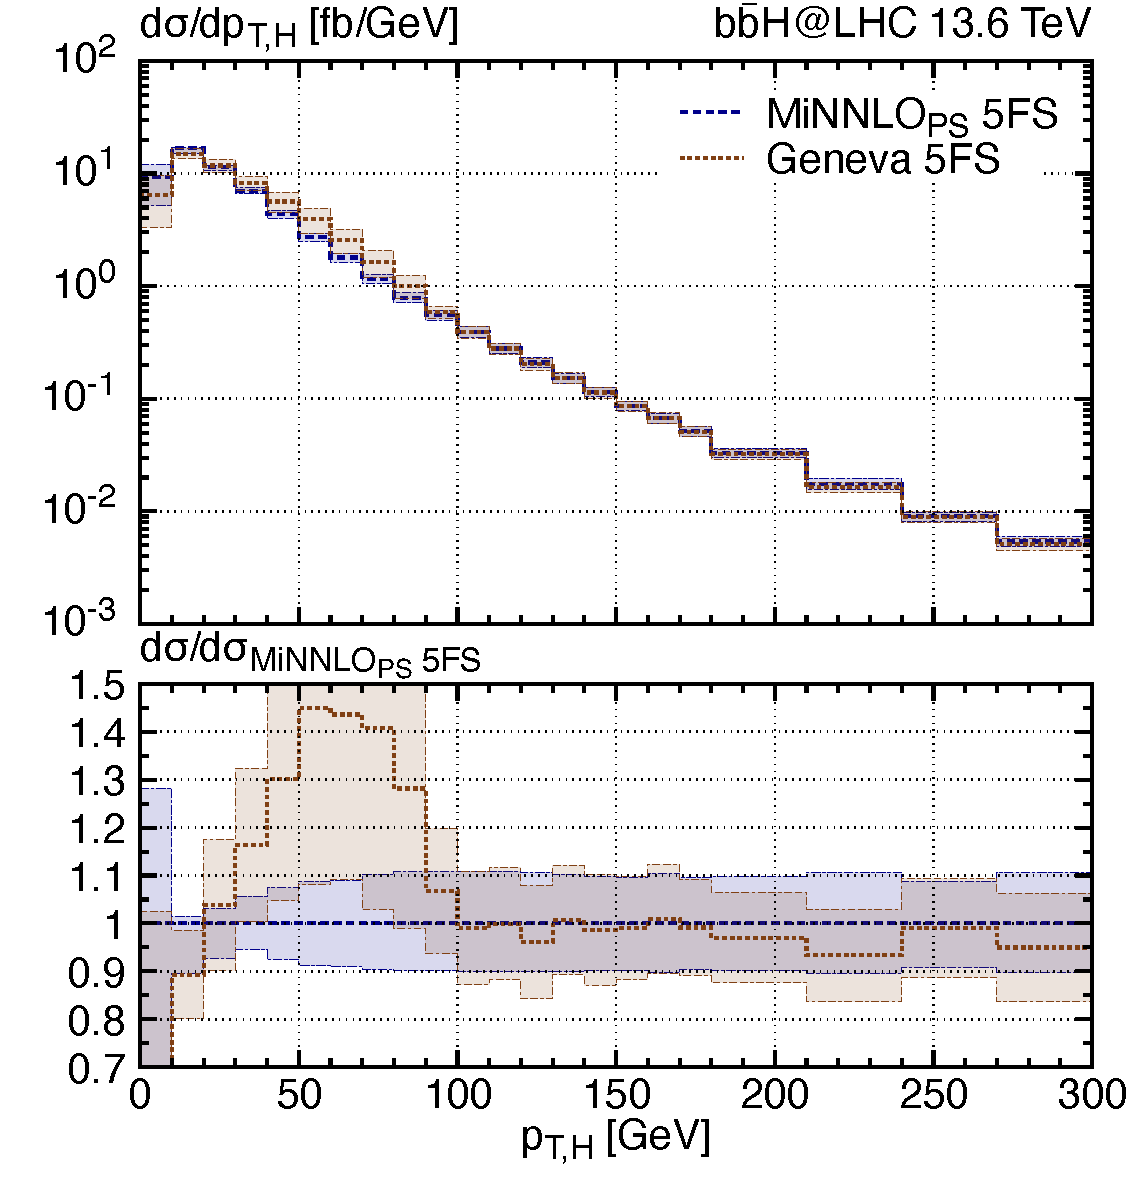
\includegraphics[width=.45\textwidth, page=1]{plots/5fs/genevaminnlo/minnloKQvar-geneva-ptH.pdf}&
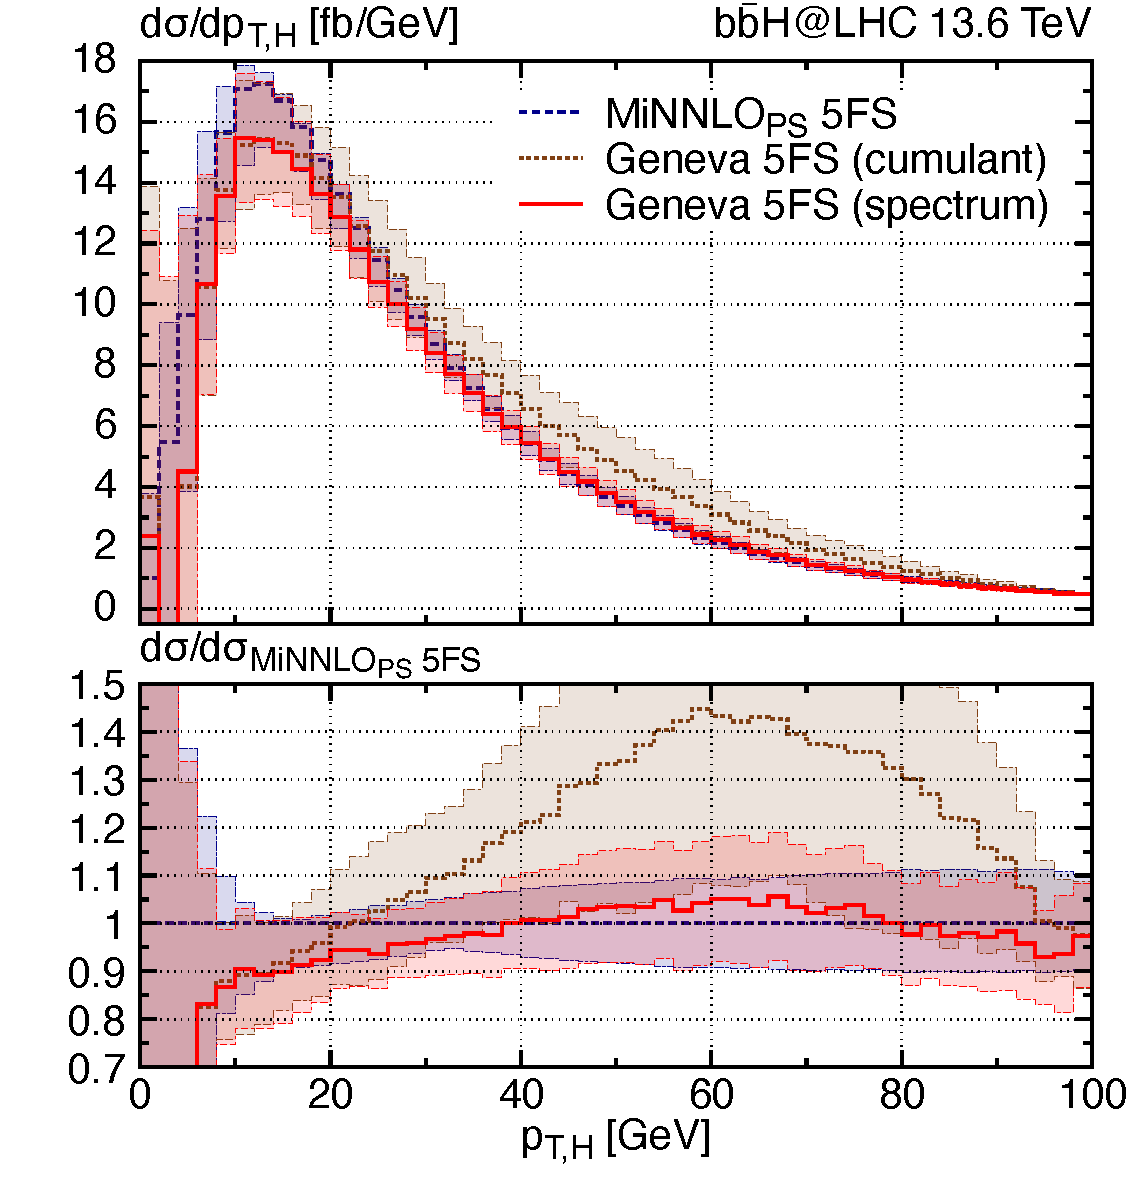
\includegraphics[width=.45\textwidth, page=1]{plots/5fs/genevaminnlo/minnloKQvar-genevaspec-ptHzoom.pdf}
\end{tabular}
\vspace*{1ex}
\caption{Comparison of \minnlo{} (blue, dashed) and \GENEVA{} (brown, dotted) predictions at NNLO+PS level for the transverse momentum distribution of the Higgs boson. The zoom version shows an alternative scale choice of the \GENEVA{} generator (red, solid).\label{fig:genevaptH}}
\end{center}
\end{figure}

\begin{figure}[t!]
\begin{center}
\begin{tabular}{cc}
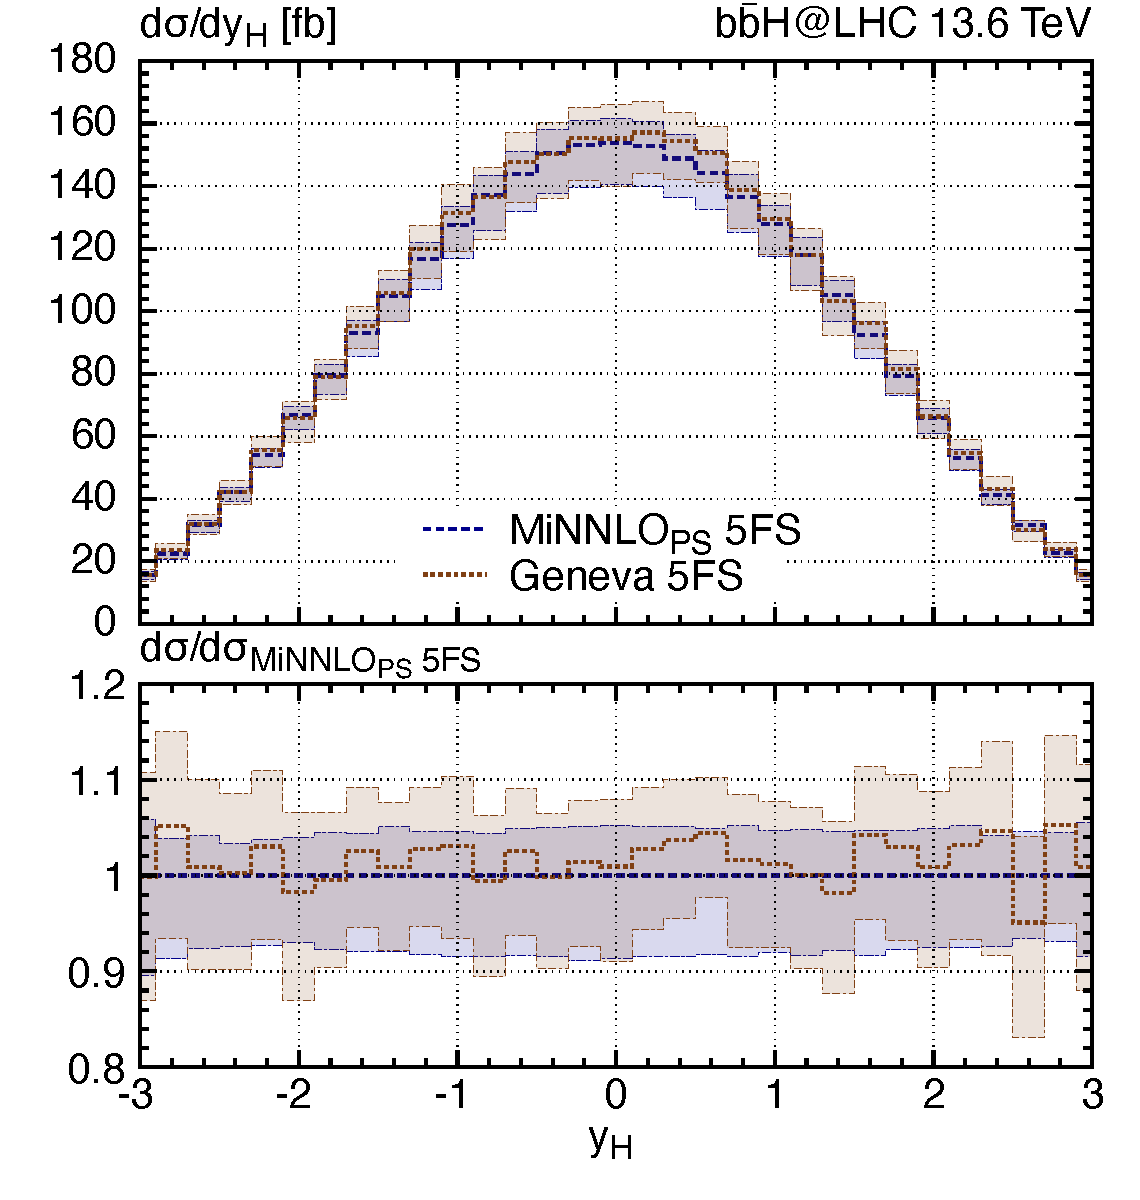
\includegraphics[width=.45\textwidth, page=1]{plots/5fs/genevaminnlo/minnloKQvar-geneva-yh.pdf}&
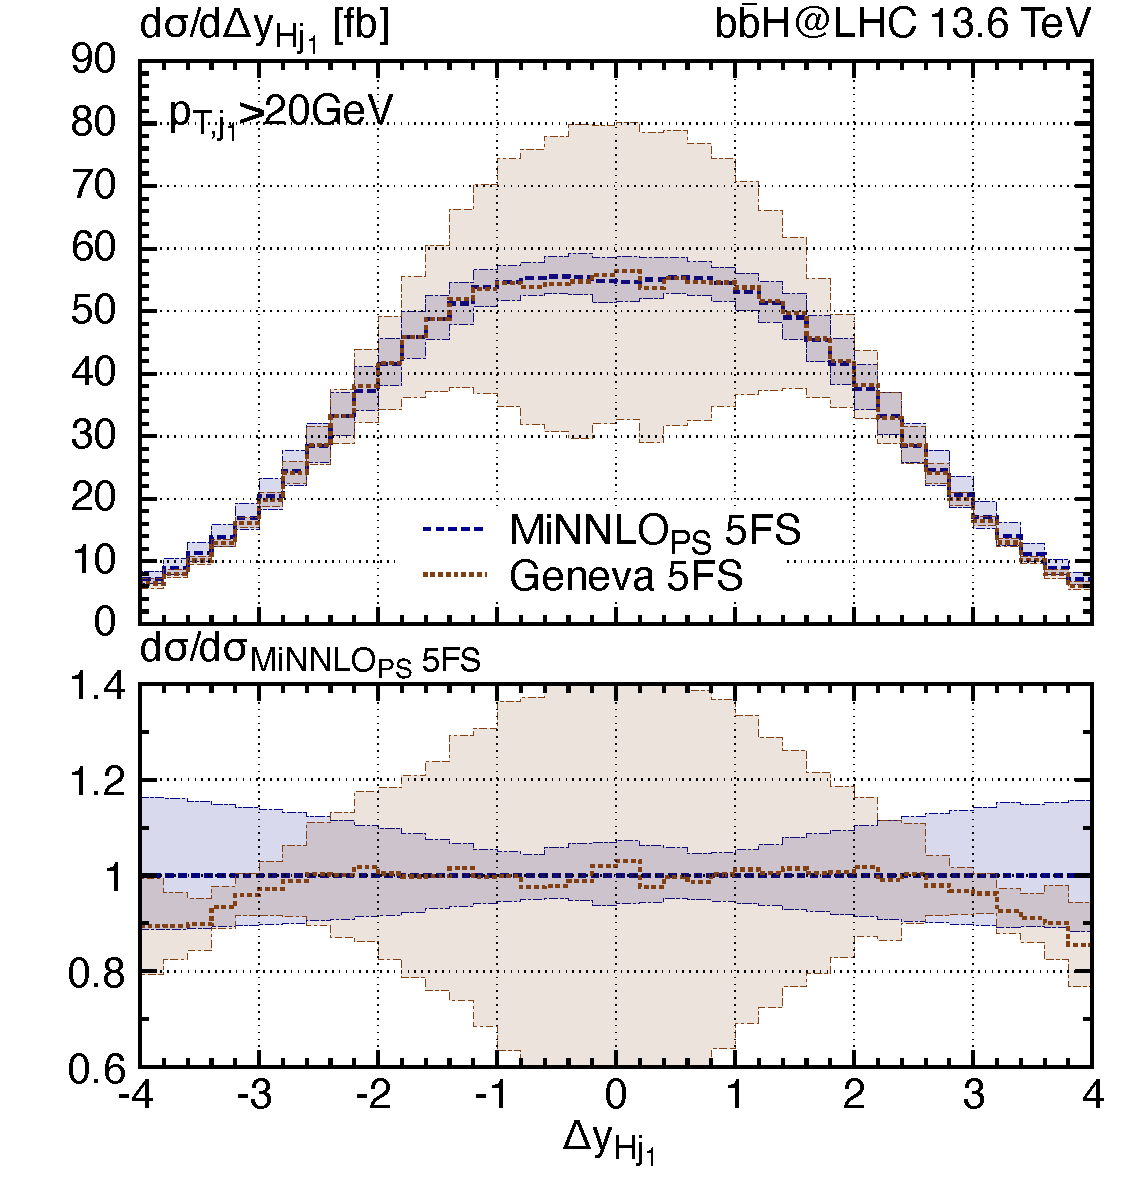
\includegraphics[width=.45\textwidth, page=1]{plots/5fs/genevaminnlo/minnloKQvar-geneva-dyhj.pdf}
\end{tabular}
\vspace*{1ex}
\caption{Higgs boson rapidity and difference in rapidity between the scalar and the leading jet as predicted by two Monte Carlo generators interfaced with \PYTHIA8{} using the \minnlo{} (blue, dashed) and \GENEVA{} (brown, dotted) methods. \label{fig:genevay}}
\end{center}
\end{figure}

\subsubsection{Transverse-momentum spectrum against resummed predictions}

\subsubsection{Heavy-Higgs for BSM studies in \minnlo{}}

The Higgs production in association with a bottom-quark pair is of particular interest in extensions beyond the Standard Model. Indeed, many BSM scenarios predict modifications to the Higgs-bottom quark coupling, which could lead to observable deviations in the production rates and kinematic distributions of the \bbH{} process. In some models, \bbH{} can become the dominant production mode of exotic Higgs states. The \minnlo{} generator presented in section~\ref{sec:5FSNNLOPS} is built within the Standard Model framework, but can be easily extended to accommodate BSM predictions. To illustrate its potential, we consider a specific example of how the NNLO+PS generator can be adapted for BSM scenarios. We specifically consider the Minimal Supersymmetric Standard Model (MSSM)~\cite{Ovrut:1984uc,Haber:1984rc,Gunion:1984yn}, which corresponds to a Type-II Two-Higgs-Doublet Model (2HDM)~\cite{Branco:2011iw} at leading order but deviates from it at higher orders. MSSM enforces relations between the Higgs sector and the superpartners of SM particles. Unlike the SM, the MSSM requires two Higgs doublets ($H_u$ and $H_d$) to give mass to both up-type and down-type fermions. An important parameter of the model is the ratio of vacuum expectation values ($v_u$ and $v_d$) of the two SU(2) doublets,
\begin{align}
	\tan\beta=\frac{v_u}{v_d}\,.
\end{align}
The other indipendent parameter is the CP-even Higgs mixing angle $\alpha$. This results in five physical Higgs bosons: two CP-even (H,H'), one CP-odd (A) and two charged Higgs bosons ($\text{H}^{\pm}$). The lightest Higgs boson ($\text{H}$) in MSSM can mimic the SM Higgs, but has different properties depending on model parameters. The tree-level mass of $\text{H}$ is bounded from above by $m_Z |\cos 2\beta|$, where $m_Z$ is the Z-boson mass. However, radiative corrections (mainly from the SUSY partners of the bottom and top quarks) can significantly alter the tree-level prediction, allowing for $m_H\sim 125$ GeV~\cite{Heinemeyer:2011aa,Bechtle:2012jw,Draper:2016pys,Bechtle:2016kui,Haber:2017erd}. We perform the NNLO+PS prediction in the benchmark configuration known as $M_H^{125}$ scenario~\cite{Bagnaschi:2018ofa}, where all superparticles are chosen to be so heavy that the presence of these effects has only a mild impact on the production and decay of MSSM Higgs bosons. As a result, the phenomenology of this scenario at the LHC closely resembles that of a Type-II 2HDM with Higgs couplings inspired by the MSSM. For the chosen mass of the supersymmetric partners, we refer to eq. (4) of~\citere{Bagnaschi:2018ofa}. SUSY particles affect the bottom Yukawa coupling, encoded on the resummation of loop-induced effects, which are $\tan\beta$-enhanced. We stress that the NNLO+PS calculation in the massless scheme contains only terms proportional to the squared bottom Yukawa coupling. As a result, predictions in the MSSM scenario differ from those in the SM solely by an overall rescaling factor. In the case of the CP-odd Higgs production, we have:
\begin{align}
	\dd \sigma_{b\bar b \text{A}}^{\text{MSSM}} = \dd \sigma_{\bbH{}}^{\text{SM}} \cdot (\tilde g_b^{\phi})^2\,,	\label{eq:BSMYuk}
\end{align}
with
\begin{align}
	\tilde{g}_b^A = \frac{\tan \beta}{1 + \Delta_b} \left( 1 - \Delta_b \frac{1}{\tan^2\beta} \right)\,.
\end{align}
The parameter \( \Delta_b \) resums higher-order sbottom contributions~\cite{Banks:1987iu,Hall:1993gn,Carena:1994bv,Carena:2000uj}. Electroweak corrections from neutralinos and charginos are incorporated into \( \Delta_b \) for this benchmark, with its numerical value determined by \texttt{FeynHiggs}~\cite{Heinemeyer:1998yj,Bahl:2018qog}. 
%The parameters \( g_f^\phi \) represent the genuine Yukawa couplings, which depend on the two angles governing the Higgs-matter interactions as defined in~\tab{tab:MSSMcoup}.\\
%\begin{table}[h]
%    \centering
%    \begin{tabular}{|c|c|c|}
%        \hline
%        \textbf{Coupling} & \textbf{MSSM value} \\
%        \hline
%        $g_u^H$ &  $\cos\alpha / \sin\beta$ \\
%        $g_d^H$ &  $-\sin\alpha / \cos\beta$ \\
%        $g_u^{H'}$ & $\sin\alpha / \sin\beta$ \\
%        $g_d^{H'}$ & $\cos\alpha / \cos\beta$ \\
%        $g_u^A$ & $\cot\beta$ \\
%        $g_d^A$ & $\tan\beta$ \\
%        \hline
%    \end{tabular}
%    \caption{Relative couplings $g_f^\phi$ with respect to the SM Yukawa coupling. The bottom Yukawa values correspond to the down-type couplings.}\label{tab:MSSMcoup}
%\end{table}
As indicated by the current constraints on \( M_H^{125} \) scenario, we consider the case of a CP-odd Higgs with a mass of 1.4 TeV and \( \tan\beta = 20 \), a point in the parameter space which is currently not excluded. In this scenario, the lightest Higgs has a mass consistent with experimental observations. We have performed the predictions by running the \minnlo{} 5FS generator with a heavy Higgs-boson mass and adjusted the Yukawa coupling according to~\eqn{eq:BSMYuk}.

\begin{figure}[t!]
\begin{center}
\begin{tabular}{cc}
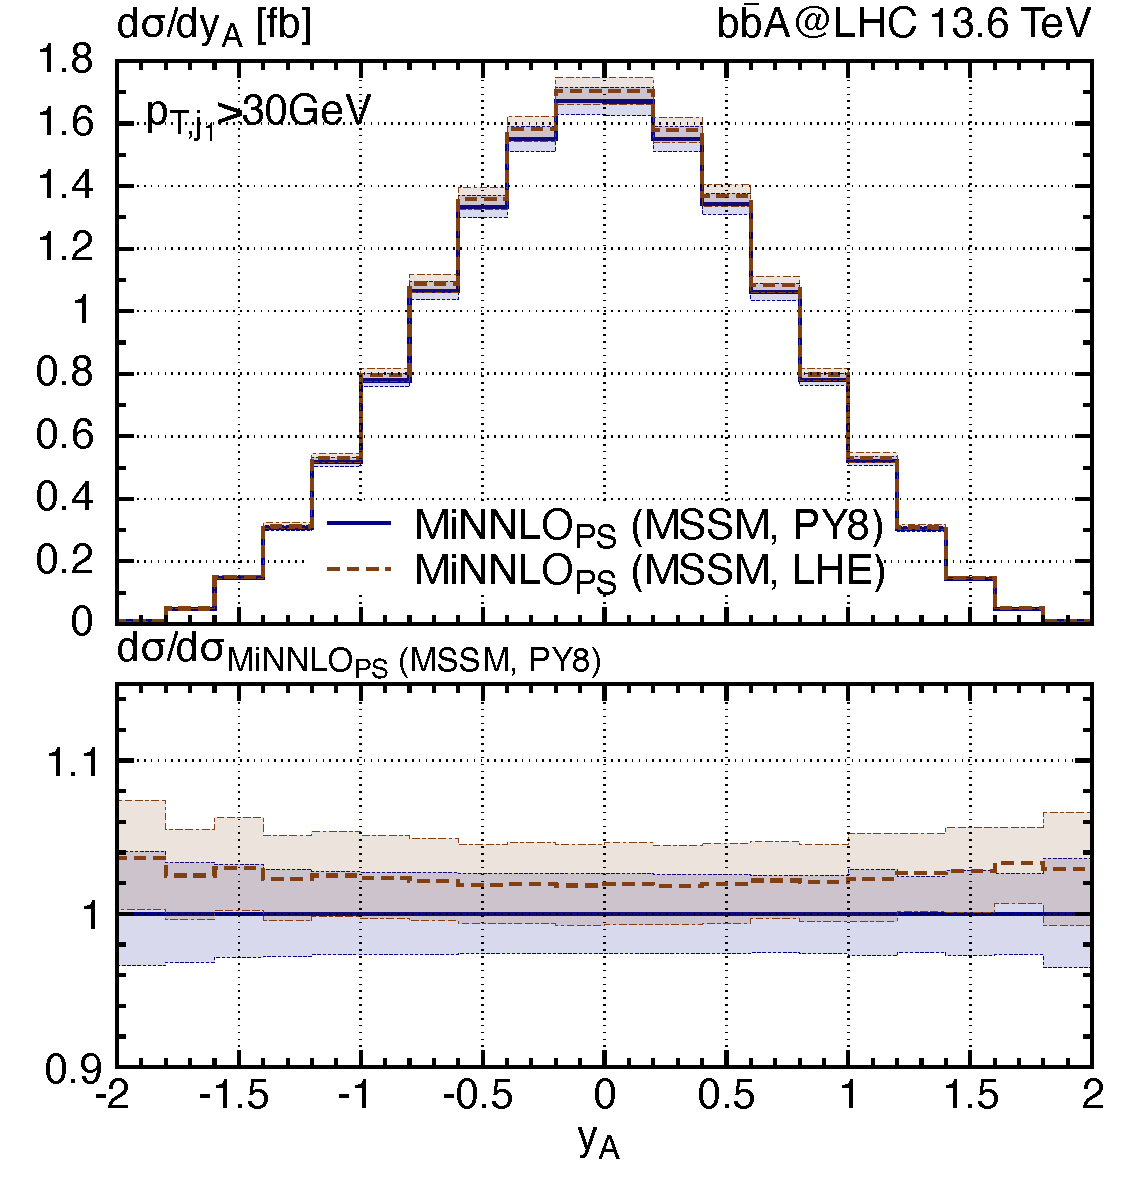
\includegraphics[width=.45\textwidth, page=1]{plots/5fs/BSM/y_H-ptj30__A-1400GeV-.pdf}&
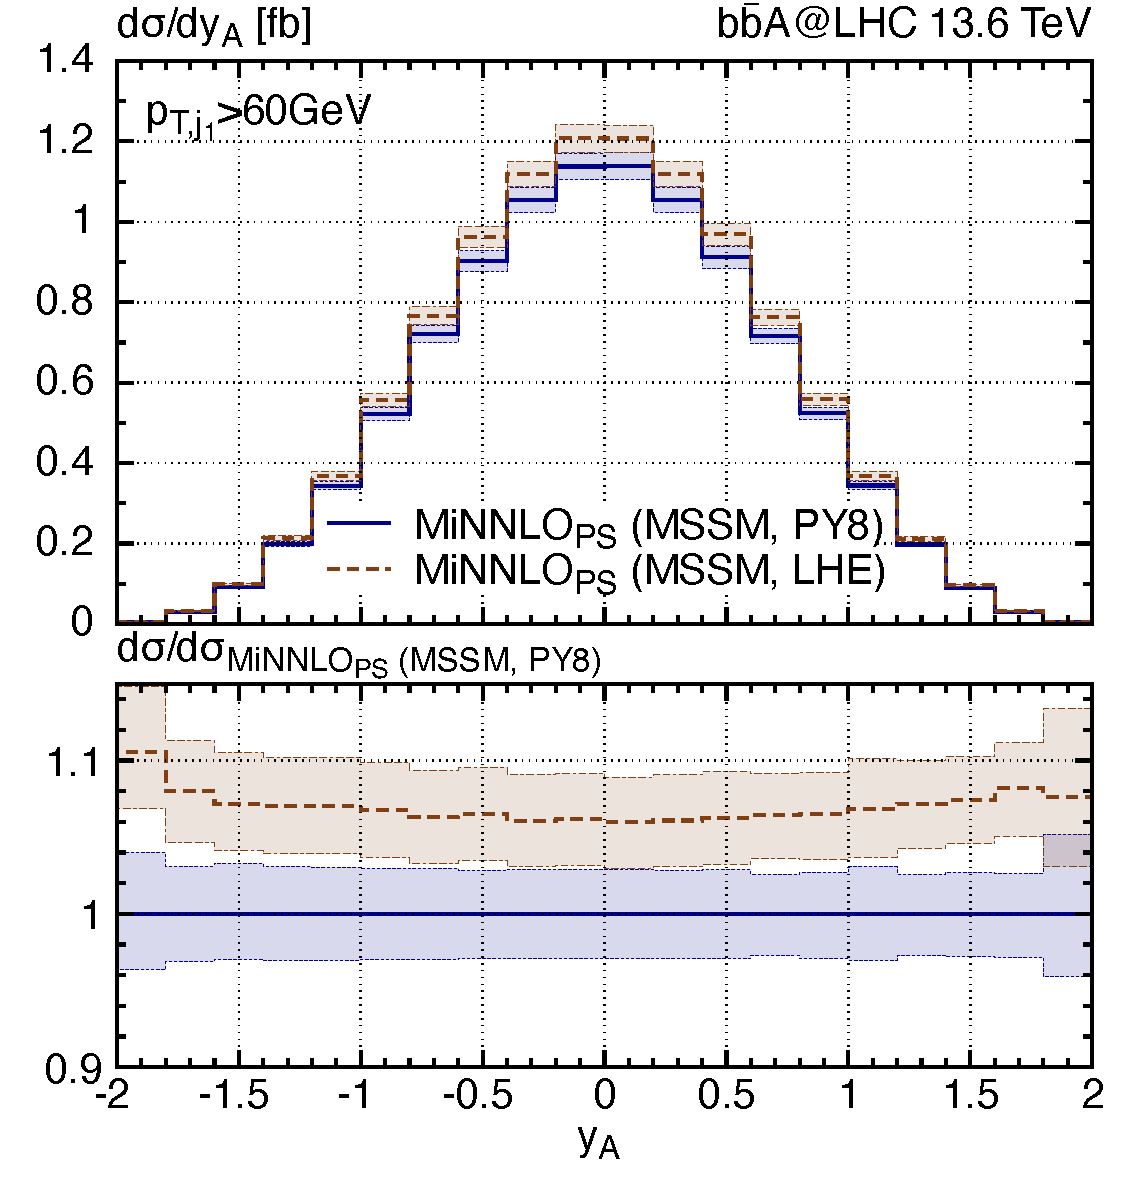
\includegraphics[width=.45\textwidth, page=1]{plots/5fs/BSM/y_H-ptj60__A-1400GeV-.pdf}
\end{tabular}
\vspace*{1ex}
\caption{Comparison of \minnlo{} results before (LHE) and after (PY8) parton shower for CP-odd Higgs rapidity spectrum. \label{fig:yA}}
\end{center}
\end{figure}

\begin{figure}[t!]
\begin{center}
\begin{tabular}{cc}
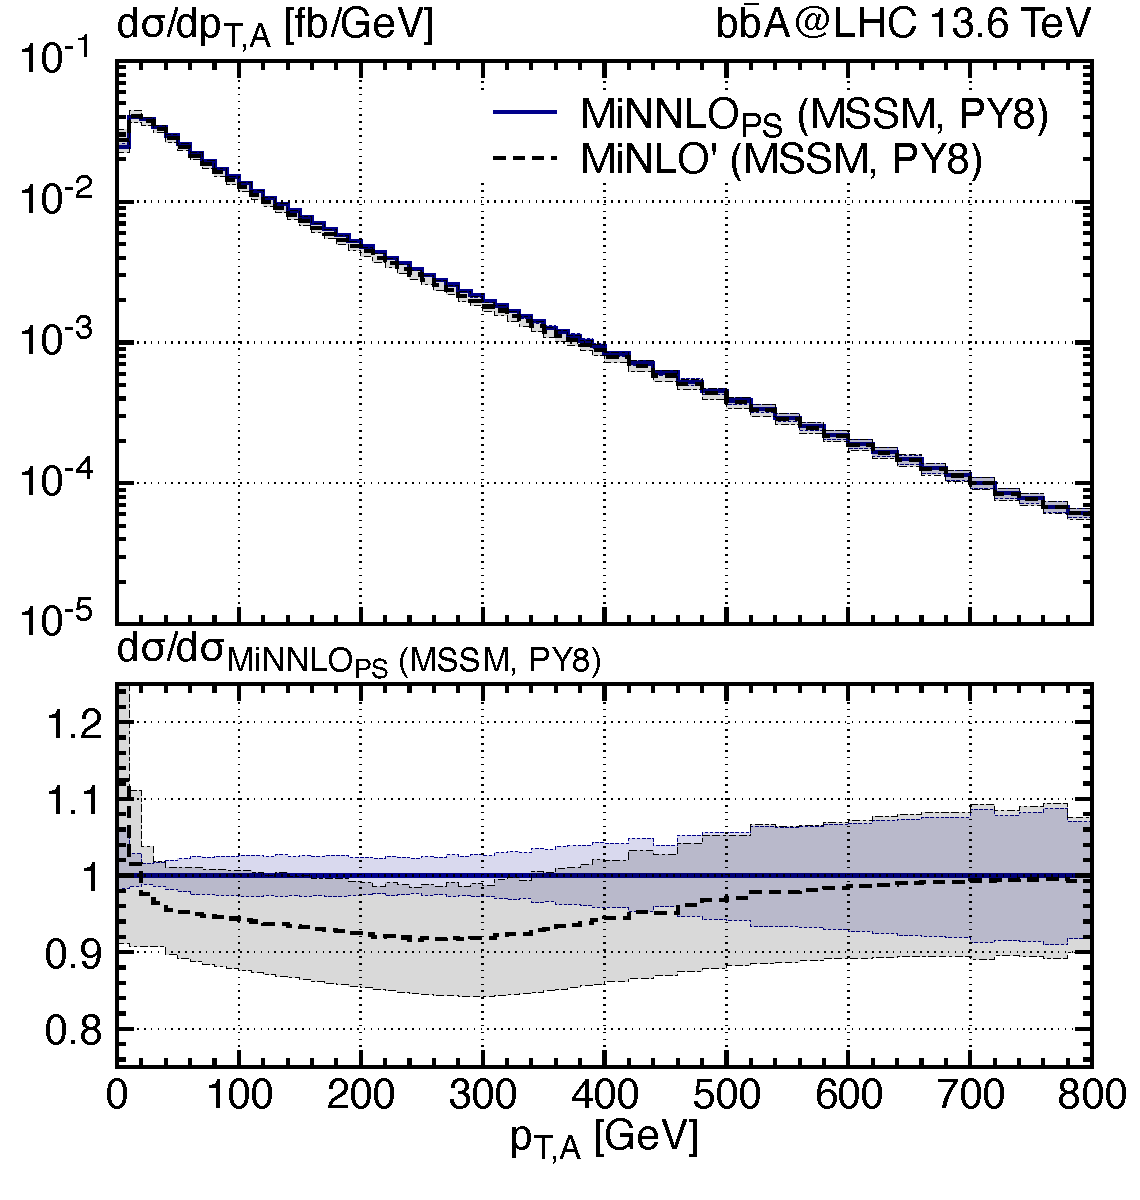
\includegraphics[width=.45\textwidth, page=1]{plots/5fs/BSM/pt_Higgs__A-1400GeV-PY8-kQ0.pdf}&
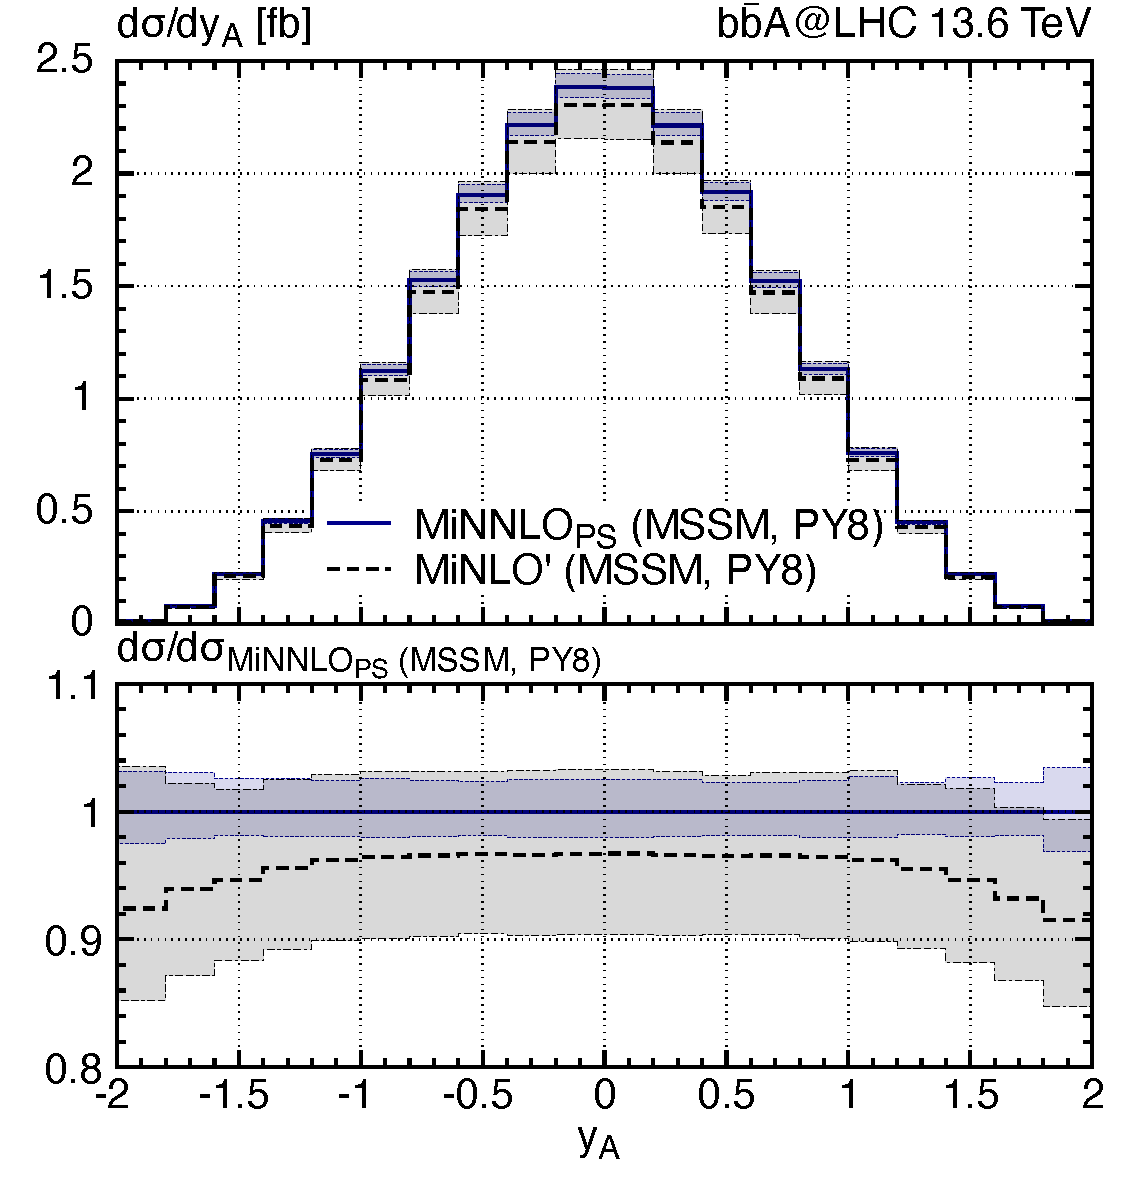
\includegraphics[width=.45\textwidth, page=1]{plots/5fs/BSM/y_Higgs__A-1400GeV-PY8-kQ0.pdf}
\end{tabular}
\vspace*{1ex}
\caption{Comparison of \minlo{} and \minnlo{} results for CP-odd Higgs rapidity spectrum with $m_A=1.4$ TeV and $\tan\beta=20$. \label{fig:MiNLOBSM}}
\end{center}
\end{figure}

\begin{figure}[t!]
\begin{center}
\begin{tabular}{cc}
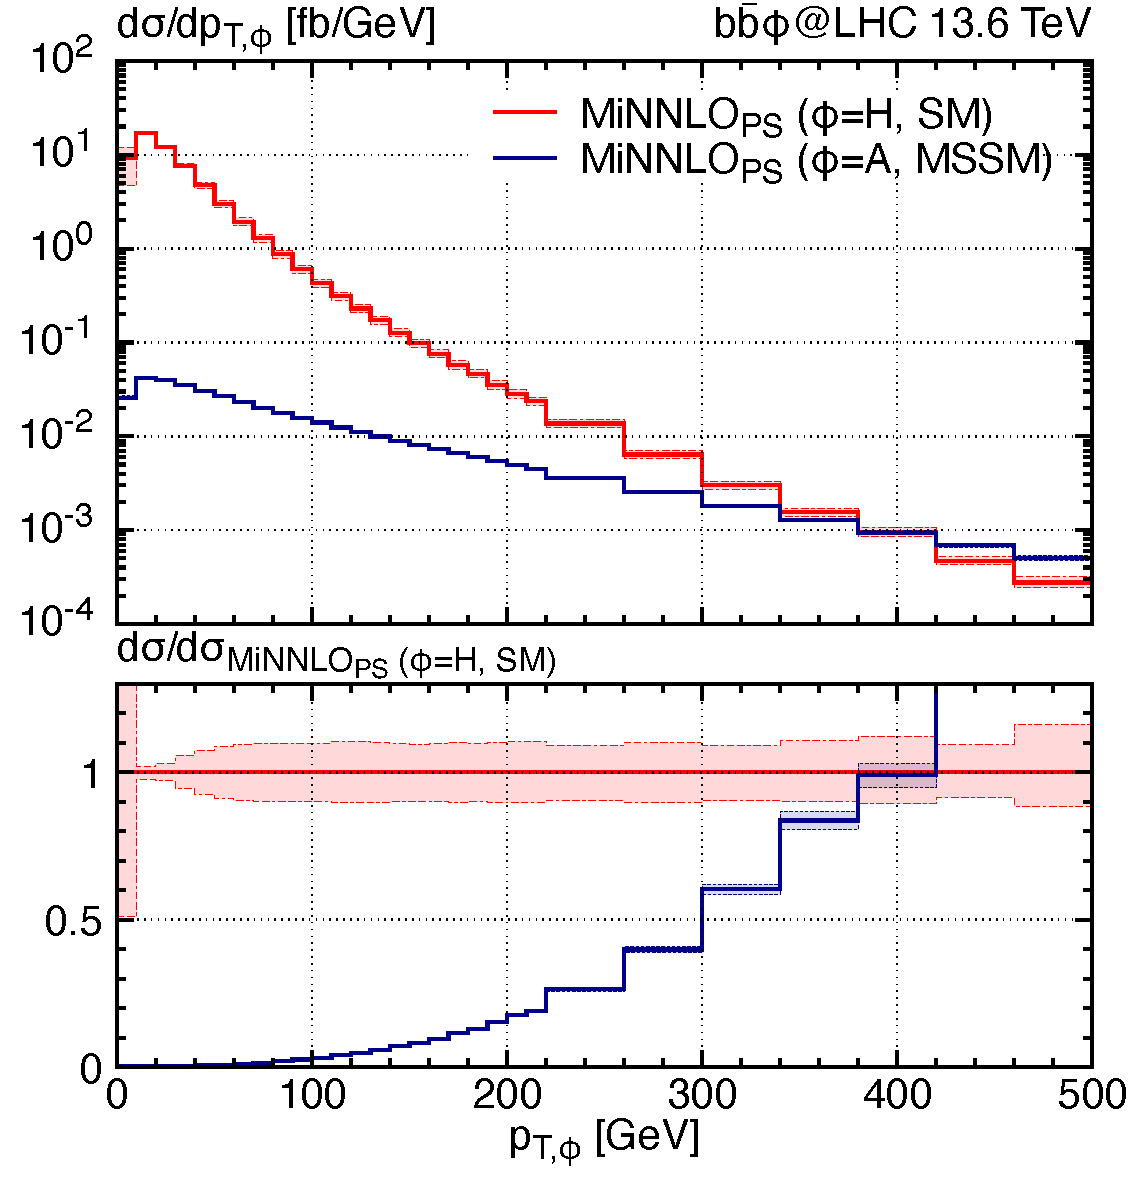
\includegraphics[width=.45\textwidth, page=1]{plots/5fs/BSM/pt_Higgs.pdf}&
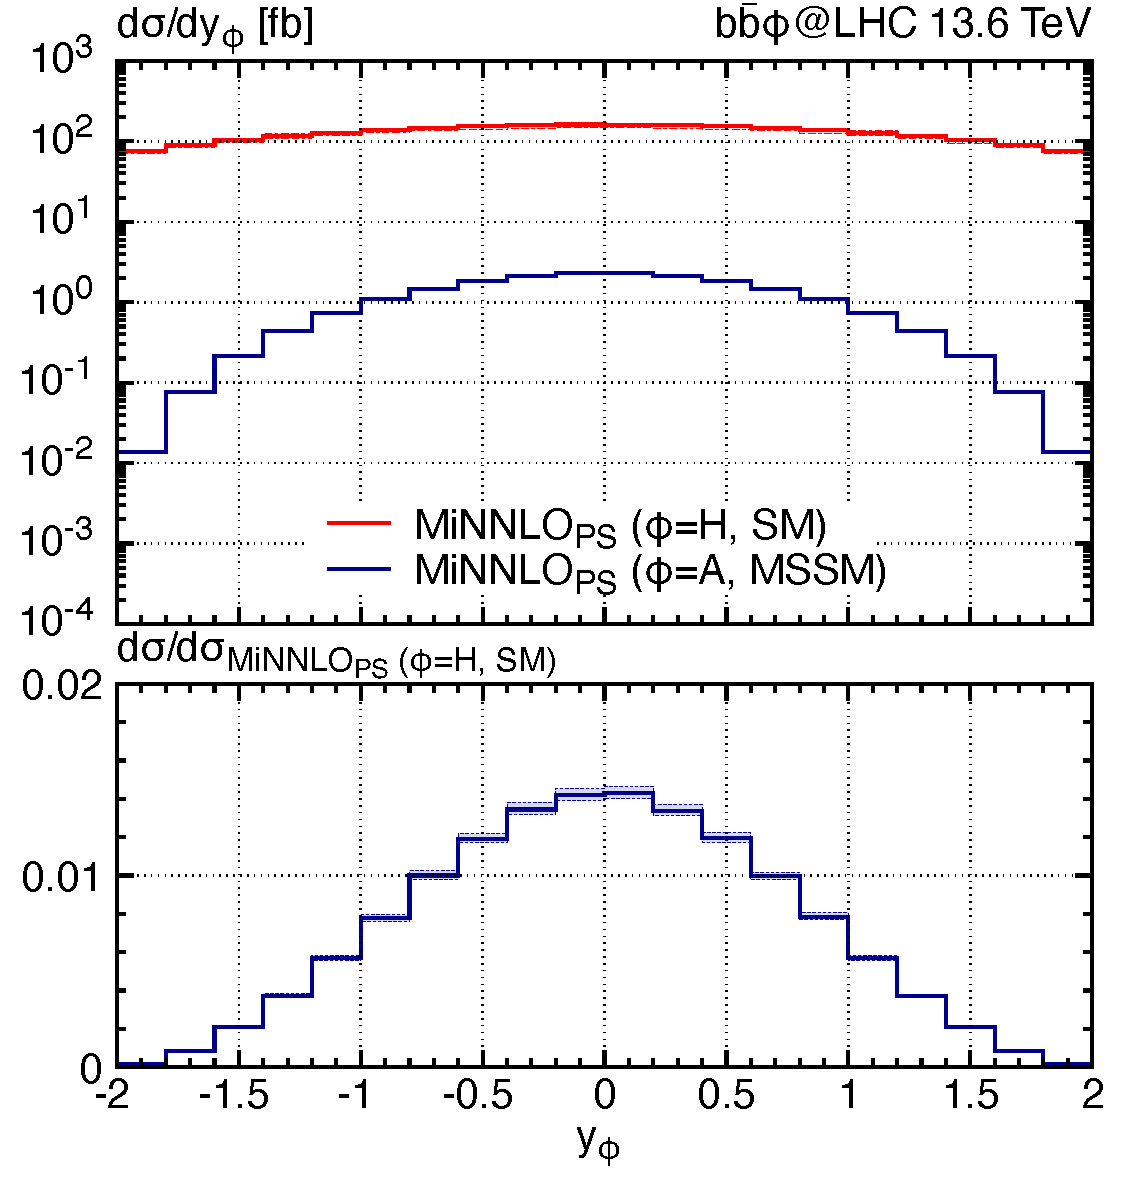
\includegraphics[width=.45\textwidth, page=1]{plots/5fs/BSM/y_Higgs.pdf}
\end{tabular}
\vspace*{1ex}
\caption{Higgs transverse momentum and rapidity spectra for \minnlo{} results with the heavy CP-odd Higgs $\text{A}$ compared to SM predictions.\label{fig:SMvsBSM}}
\end{center}
\end{figure}

In~\fig{fig:yA}, we present a comparison of the rapidity distribution of the Higgs boson A in an exclusive phase-space region. We compare the results before and after interfacing the LHE events with Pythia 8. The jet spectrum becomes slightly harder after the shower. Consequently, the NNLO+PS prediction leads to higher rapidity spectra in the presence of a transverse momentum cut of 30 GeV and 60 GeV for the leading jet. As expected, we verified that in the absence of jet cuts, the shower does not change the Higgs rapidity.  

We now turn to~\fig{fig:MiNLOBSM}, where we present a comparison between \minnlo{}  and \minlo{} predictions for the CP-odd Higgs. Due to the high mass of the bosonic state, the resummation region extends over a broader range of the transverse momentum spectrum compared to the SM Higgs, with a mass of 125 GeV. As a result, the NNLO corrections present in \minnlo{} have a greater impact even at intermediate transverse momentum values, leading to more accurate predictions and smaller scale uncertainties compared to the \minlo{} ones. In the second plot of~\fig{fig:MiNLOBSM}, we compare the two predictions for the Higgs rapidity spectrum: NNLO corrections increase the cross-section while having a flat effect in the central region $|y_A|<1$. Notably, the NNLO effects encoded in \minnlo{} are positive in the case of heavy-Higgs mass, compared to the SM case where the authors of~\citere{Biello:2024vdh} have observed a flat negative correction in the Higgs rapidity spectrum.

Finally, we compare the differential behaviour of \minnlo{} predictions for the heavy Higgs state with the SM distributions in~\fig{fig:SMvsBSM}. As expected, the BSM transverse momentum spectrum is harder. With the chosen settings, BSM effects become at least half as large as, or even larger than, the SM effects for transverse-momentum values greater than 300 GeV. In the right plot of~\fig{fig:SMvsBSM}, we compare the rapidity distributions. The heavy CP-odd Higgs exhibits a spectrum more concentrated at small rapidity values, with its contribution remaining always below 2\% of the SM prediction. We stress that the numerical comparison is highly sensitive to the choice of the MSSM parameters. However, the purpose of this analysis is not to focus on a specific choice of the MSSM parameters, but to demonstrate the potential of the \minnlo{} generator for BSM modeling of \bbH{} production at NNLO+PS.

\subsection{Bottom-Yukawa squared contribution at NNLO+PS in 4FS}\label{sec:bbH4FS}
Building on the \minnlo{} matching for \bbH{} in the massless 5FS described in Section~\ref{sec:5FSNNLOPS}, we now turn to an analogous construction in the massive 4FS that captures the \(y_{b}^{2}\) component at NNLO+PS. 
%In Section~\ref{sec:FONLLmatch}, the fixed-order FONLL combination ensured that inclusive 5FS and 4FS cross sections are consistently merged, but it left open the question of how to retain full bottom-mass dependence in a fully differential, shower-matched prediction.
Section~\ref{sec:5FSNNLOPS} demonstrated that, in 5FS, the \minnlo{} and \GENEVA{} procedures provide fully exclusive NNLO+PS results for the \bbH{} process with massless bottom quarks. While that approach naturally resums all collinear logarithms and reproduces the correct small-\(p_{T}\) behavior for the Higgs, it cannot account for finite-\(m_{b}\) recoil or reliably model observables that depend on the kinematics of hard \(b\)-jets.

\begin{comment}
To address these shortcomings, we now introduce a fully exclusive NNLO+PS generator for the \bbH{} process in the massive 4FS.  This construction follows the extension of the \minnlo{} method to heavy-quark–associated colour-singlet production (\(Q\bar{Q}F\)) developed in \cite{mazzitelli:2024ura}, which itself builds on the \minnlo{} approach for \(Q\bar{Q}\) production introduced in \cite{mazzitelli:2020jio,mazzitelli:2021mmm}.  While the pattern of large logarithms in the \(Q\bar{Q}F\) final state closely mirrors that of \(Q\bar{Q}\) production at small transverse momentum, the \(Q\bar{Q}F\) kinematics are more general—unlike in pure \(Q\bar{Q}\) production, where the heavy quarks appear back-to-back at Born level.  In both cases, one begins from the factorisation theorem in Fourier–conjugate (impact-parameter or \(b\)) space \cite{Zhu:2012ts,Li:2013mia,Catani:2014qha,Catani:2018mei}:
\begin{align}\label{eq:facformula}
        \frac{\mathd \sigma}{ \mathd^2\vec{\pt}\, \mathd \Phi_{Q\bar{Q}{\rm F}}}&=\sum_{c=q,\bar{q},g}
  \frac{|M^{(0)}_{c\bar{c}}|^2}{2 m_{Q\bar{Q}{\rm F}}^2 }\int\frac{ \mathd^2\vec{b}}{(2\pi)^2} e^{i \vec{b}\cdot
  \vec{\pt} } e^{-S_{c\bar{c}} \left(\frac{b_0}{b}\right)}\sum_{i,j} \Tr({\mathbf H}_{c\bar{c}}{\mathbf \Delta})\,\,
  ({C}_{ci}\otimes f_i) \,({C}_{\bar{c} j}\otimes f_j) \,,
\end{align}
where $b_0=2 e^{-\gamma_\text{E}}$. The factor $e^{-S_{c\bar{c}}}$ represents the same Sudakov radiator that appears in the small-$p_{T}$ resummation for any colour-singlet system.  In Eq.~\eqref{eq:facformula}, the sum over $c=q,\bar{q},g$ spans all possible flavour assignments for the incoming partons, with first parton carrying flavour $c$ and the second parton carrying flavour $\bar{c}$. The collinear coefficient functions
$C_{ij} = C_{ij}\bigl(z,\,p_{1},\,p_{2},\,\vec{b};\,\alpha_{s}(b_{0}/b)\bigr)$
encode the constant terms arising from collinear emissions, and the parton densities $f_{i}$ are evaluated at the scale $b_{0}/b$.  The composite factor
$\Tr\bigl({\mathbf H}_{c\bar{c}}\,{\mathbf \Delta}\bigr)\;\bigl(C_{ci}\otimes f_{i}\bigr)\;\bigl(C_{\bar{c}j}\otimes f_{j}\bigr)$
differs in its explicit form for the $q\bar{q}$ and $gg$ channels; here it is shown in symbolic form.  In particular, this factor contains a nontrivial Lorentz structure—omitted here for brevity—that generates azimuthal correlations in the collinear limit \cite{Catani:2010pd,Catani:2014qha}.

All quantities in bold face denote operators in colour space, and the trace $\Tr\bigl({\mathbf H}_{c\bar{c}}\,{\mathbf \Delta}\bigr)$
in Eq.~\eqref{eq:facformula} runs over colour indices.  The hard function \({\mathbf H}_{c\bar{c}}\) is extracted from the infrared-subtracted amplitudes for \(Q\bar{Q}F\) production, with any ambiguity in its definition corresponding to a choice of resummation scheme~\cite{Bozzi:2005wk}.  The operator \({\mathbf \Delta}\) encodes quantum interference arising from soft radiation exchanged at large angles between the initial and final states, as well as among final-state partons. It is given by ${\mathbf \Delta}={\mathbf V}^\dagger{\mathbf D}{\mathbf V}$, where
\begin{align}
\label{eq:soft}
{\mathbf V} &= {\cal
  P}\exp\left\{-\int_{b_0^2/b^2}^{m_{Q\bar{Q}F}^2}\frac{dq^2}{q^2}{\mathbf
  \Gamma}_t(\Phi_{\rm Q\bar{Q}F};\alpha_s(q))\right\}\,.%\notag\\
\end{align}
The symbol \({\cal P}\) denotes path ordering of the exponential matrix with respect to the integration variable \(q^{2}\), arranging scales from left to right in increasing order.  The anomalous dimension \(\mathbf{\Gamma}_{t}\) governs the effect of real soft radiation emitted at large angles.  Meanwhile, the azimuthal operator $\mathbf{D} \;\equiv\; \mathbf{D}\bigl(\Phi_{Q\bar{Q}F},\,\vec{b},\,\alpha_{s}\bigr)$
encodes azimuthal correlations of the \(Q\bar{Q}F\) system in the small-\(p_{T}\) limit.  Upon averaging over the azimuthal angle \(\phi\), it satisfies
$\bigl[\mathbf{D}\bigr]_{\phi} \;=\; \mathbf{1}$.
\end{comment}

To address these shortcomings, we now introduce a fully exclusive NNLO+PS generator for the \bbH{} process in the massive 4FS.  This construction follows the extension of the \minnlo{} method to heavy-quark–associated colour-singlet production (\(Q\bar{Q}F\)) developed in \citere{mazzitelli:2024ura}, which itself builds on the \minnlo{} approach for \(Q\bar{Q}\) production introduced in \cite{mazzitelli:2020jio,mazzitelli:2021mmm}. The procedure to construct a \minnlo{} improved \(\bar{B}\) function for the \(Q\bar{Q}F\) system is the same as that of the colour-singlet case, and it is based on the generation of the factorisation theorem for heavy-quark pair production \cite{Zhu:2012ts,Li:2013mia,Catani:2014qha,Catani:2018mei} in arbitrary kinematics.  All technical details of this derivation are provided in Refs.~\cite{mazzitelli:2020jio,mazzitelli:2021mmm,mazzitelli:2024ura,Biello:2024pgo}.

In the case of \bbH{} production in the 4FS, the two-loop virtual correction required for NNLO accuracy is not available in exact form with finite \(m_b\). To circumvent this, the NNLO+PS prediction relies on an approximate treatment of the two-loop amplitude: the known massless result is massified by retaining all logarithmic and constant terms, while dropping terms that are power-suppressed in \(m_b / m_{H}\). This massification procedure, developed in \citeres{Mitov:2006xs,Wang:2023qbf}, allows one to capture the dominant virtual corrections in the small-\(m_b\) limit. The massless full-colour two-loop amplitudes used as input are taken from \citere{Badger:2024mir}. Hence, the NNLO calculation is complete, except for the missing power-suppressed corrections in the bottom-quark mass of the two-loop contribution.

\subsubsection{Results}
The setup for the phenomenological results presented here—including input parameters, renormalisation and factorisation scale choices and PDFs —follows the conventions outlined in Section~\ref{sec:setup}. We now compare theoretical predictions obtained in the 5FS and 4FS for Higgs production in association with bottom quarks. The results are organised in two stages: first, we consider fully inclusive observables that do not rely on identifying bottom quarks in the final state; subsequently, we turn to observables involving b-jets, with a careful definition of flavour-tagged jets for a meaningful comparison between schemes.
\begin{table}[ht!]
  \vspace*{0.3ex}
  \begin{center}
	   \renewcommand{\arraystretch}{1.6}
    \begin{tabular}{|c||c|c|c|c|}
    \hline
    \makecell[c]{\shortstack{\rule{0pt}{2ex}Fiducial region}} &  
    \makecell[c]{\shortstack{\rule{0pt}{2ex}NLO$_{\rm PS}$ \\ 5FS} } & 
    \makecell[c]{\shortstack{\rule{0pt}{2ex}NLO$_{\rm PS}$ \\ 4FS} }  & 
    \makecell[c]{\shortstack{\rule{0pt}{2ex}\minnlo{} \\ 5FS} } &  
    \makecell[c]{\shortstack{\rule{0pt}{2ex}\minnlo{} \\ 4FS ($a2\ell_{\rm FC}$)\footnotemark} } \\
    \hline \hline
	    H & $725.(3)_{-10\%}^{+11\%}$ & $ 389.(9)_{-20\%}^{+24\%}$ & $ 575.(5)_{-8.0\%}^{+4.5\%}$ & $ 520.(9)_{-15\%}^{+19\%}$\\
     \hline
	    H $+\geq1\,bj_{\text{IFN}}$ & $105.(6)_{-10\%}^{+10\%}$ & $ 76.4(4)_{-20\%}^{+26\%}$ & $ 116.(8)_{-8.8\%}^{+9.3\%}$& $ 98.6(5)_{-12\%}^{+7.7\%}$\\
      \hline
	    H $+\geq2\,bj_{\text{IFN}}$ & $5.9(1)_{-10\%}^{+10\%} $ & $ 5.0(1)_{-23\%}^{+32\%}$ & $ 8.5(6)_{-10\%}^{+11\%}$& $ 7.0(2)_{-10\%}^{+1.6\%}$ \\
       \hline
        H $+0\,bj_{\text{IFN}}$  & $621.(1)_{-10\%}^{+11\%}$ & $ 313.(6)_{-20\%}^{+23\%}$ & $ 459.(8)_{-7.8\%}^{+3.3\%}$&$ 421.(0)_{-15\%}^{+21\%}$ \\
        \hline
    \end{tabular}
  \end{center}
  \vspace{-1em}
  \caption{
	Cross-section values in fb of the different \POWHEG{} generators in massless and massive schemes. 
	\label{tab:NNLO4FS_xs}}
\end{table}
\footnotetext{%
  ($a2\ell_{\rm FC}$) stands for approximate two-loop amplitudes, obtained by massifying the massless amplitude in the full-colour limit.
}
\begin{figure}[t!]
\begin{center}
\begin{tabular}{cc}
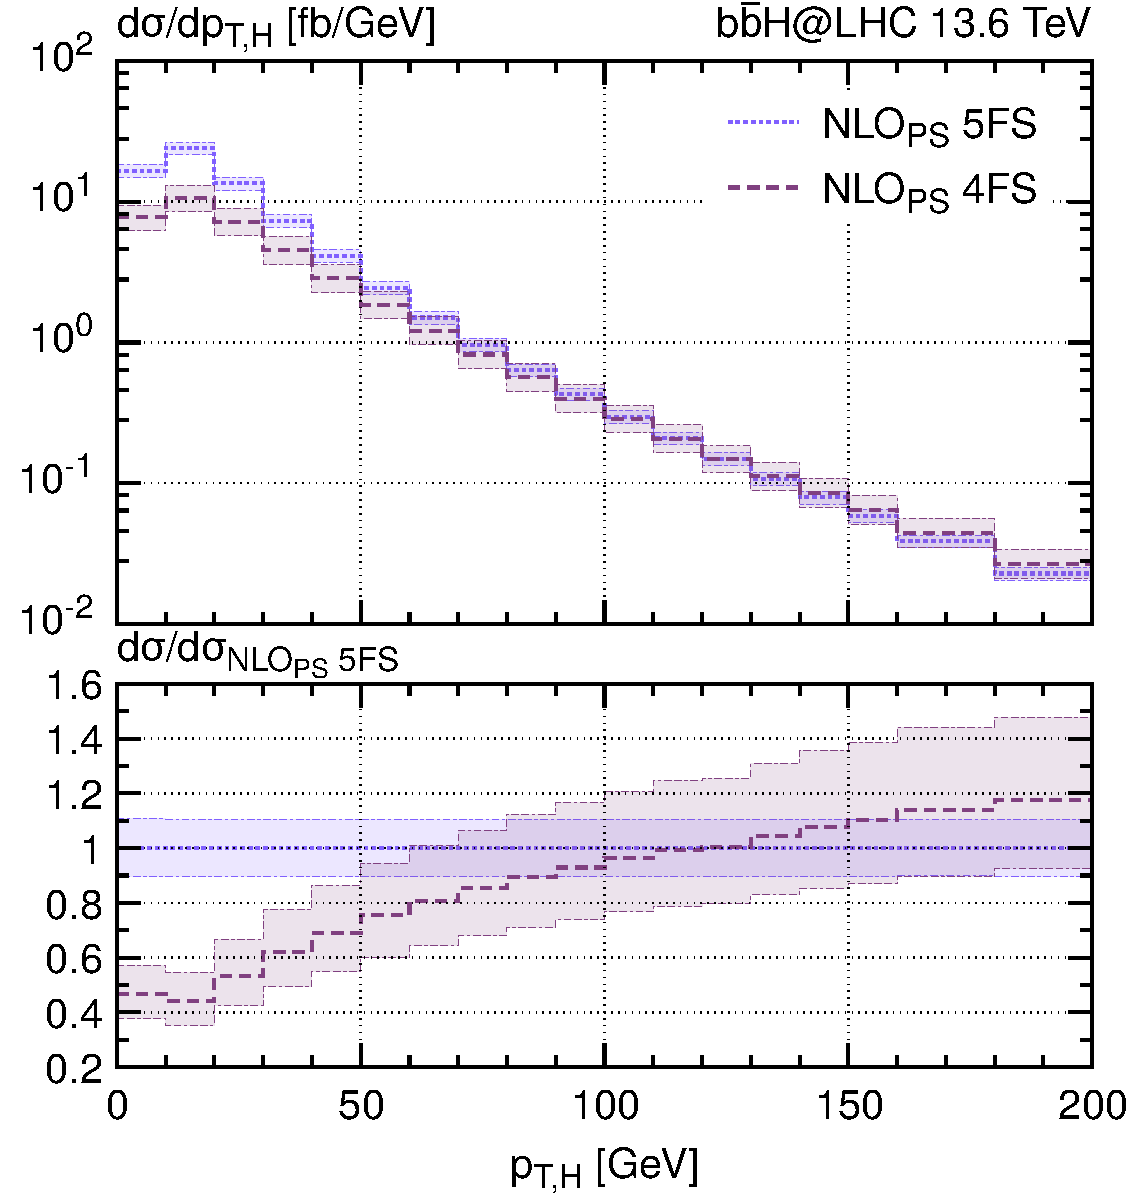
\includegraphics[width=.45\textwidth, page=1]{plots/4fs/pt_Higgs_NLO_5FS_4FS.pdf}&
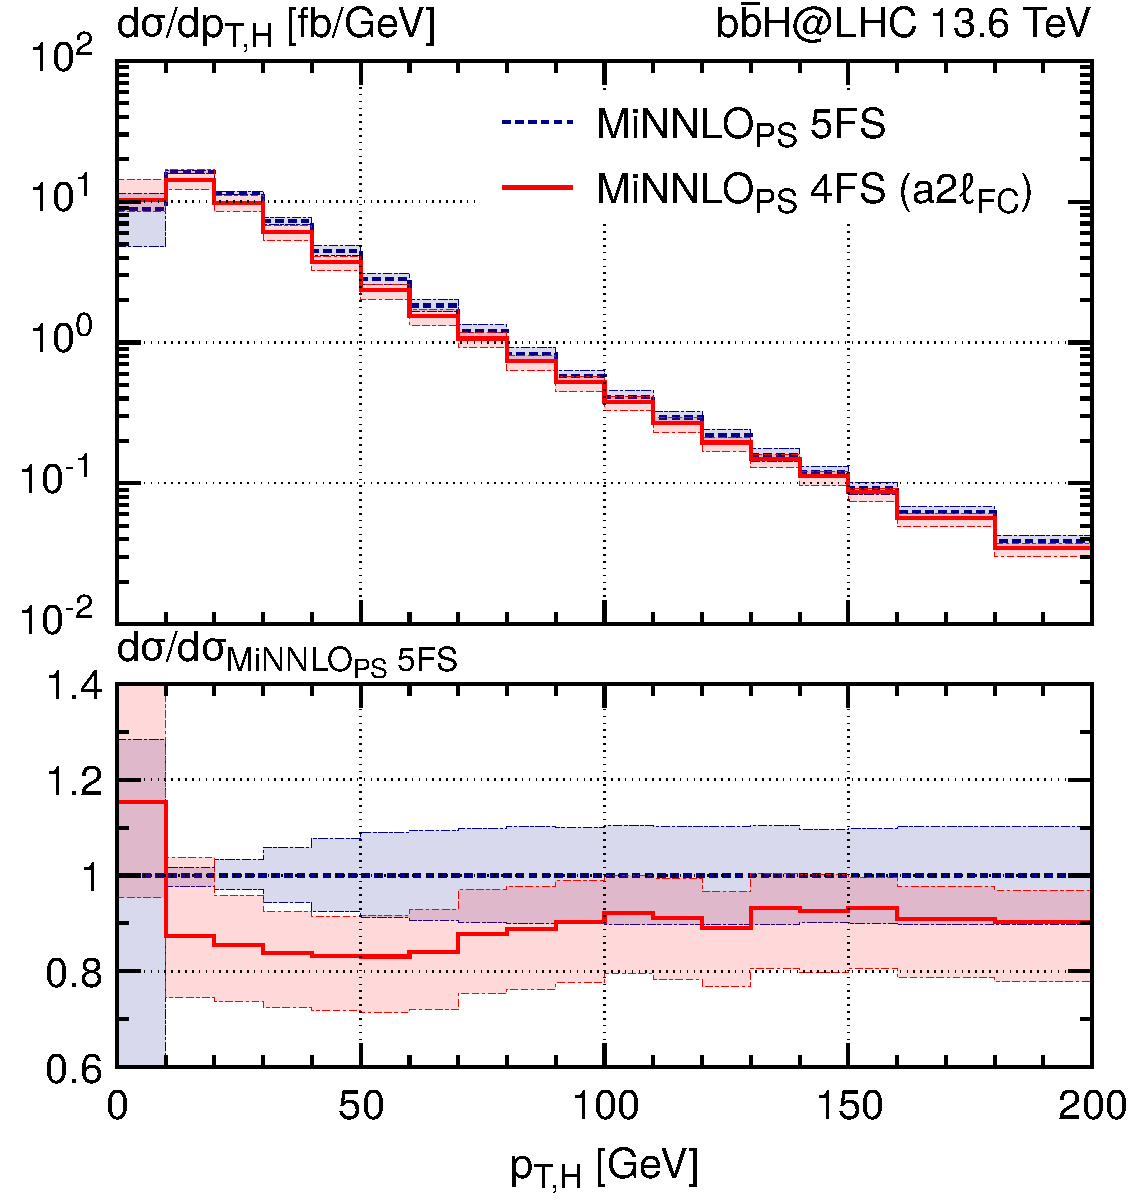
\includegraphics[width=.45\textwidth, page=1]{plots/4fs/pt_Higgs_minnlops_5FS_4FS-FC.pdf}
\end{tabular}
\vspace*{1ex}
\caption{Comparison between different flavour scheme choices for the Higgs transverse momentum spectrum at NLO+PS (left) and NNLO+PS level (right). \label{fig:4fsA}}
\end{center}
\end{figure}
\subsubsection*{Predictions for Higgs observables}
In the 4FS, NNLO corrections increase the total cross section by about 30\% relative to NLO, as shown in Table~\ref{tab:NNLO4FS_xs}. This highlights the importance of NNLO accuracy for precise predictions in the massive scheme. The \minnlo{} result in the 4FS shows reduced dependence on the scale choices as compared to the NLO+PS prediction. However, \minnlo{} prediction in the 5FS—based on the process \(b\bar{b} \to H+X\)—has a smaller scale uncertainties. 
%This difference arises from the structure of the perturbative expansion: in the 4FS, strong couplings appear already at Born level, and the NNLO corrections are relatively large.
Despite these differences, the NNLO+PS predictions in both schemes agree well within their respective scale uncertainties, demonstrating that the long-standing tension between the 4FS and 5FS inclusive results is reduced once NNLO accuracy is included.
\begin{figure}[t!]
\begin{center}
\begin{tabular}{cc}
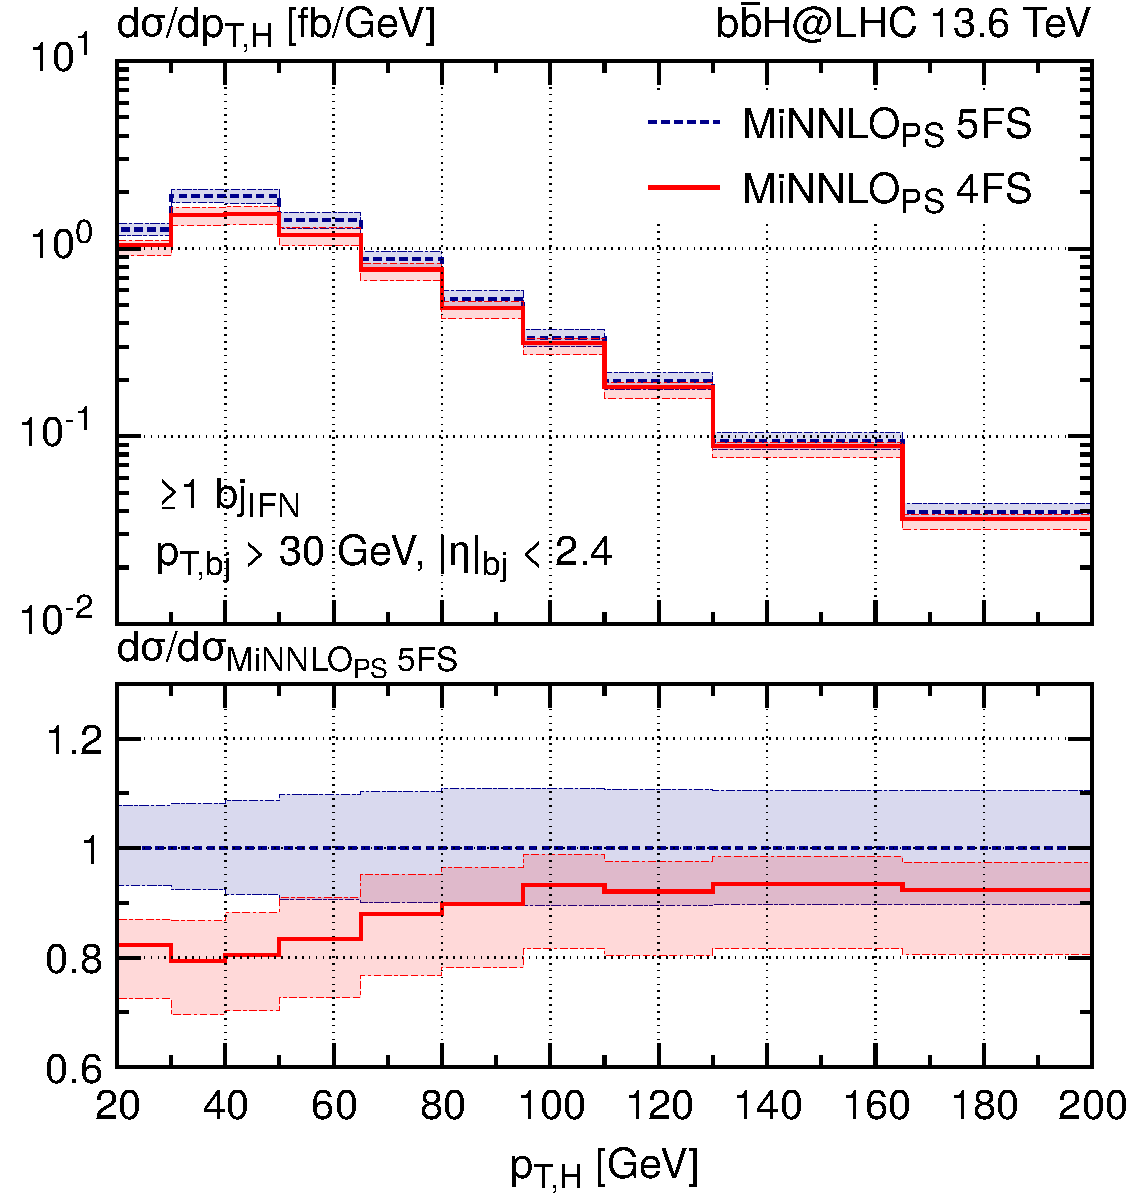
\includegraphics[width=.45\textwidth, page=1]{plots/4fs/pt_H-IFN-1bjet_minnlops-FC.pdf}&
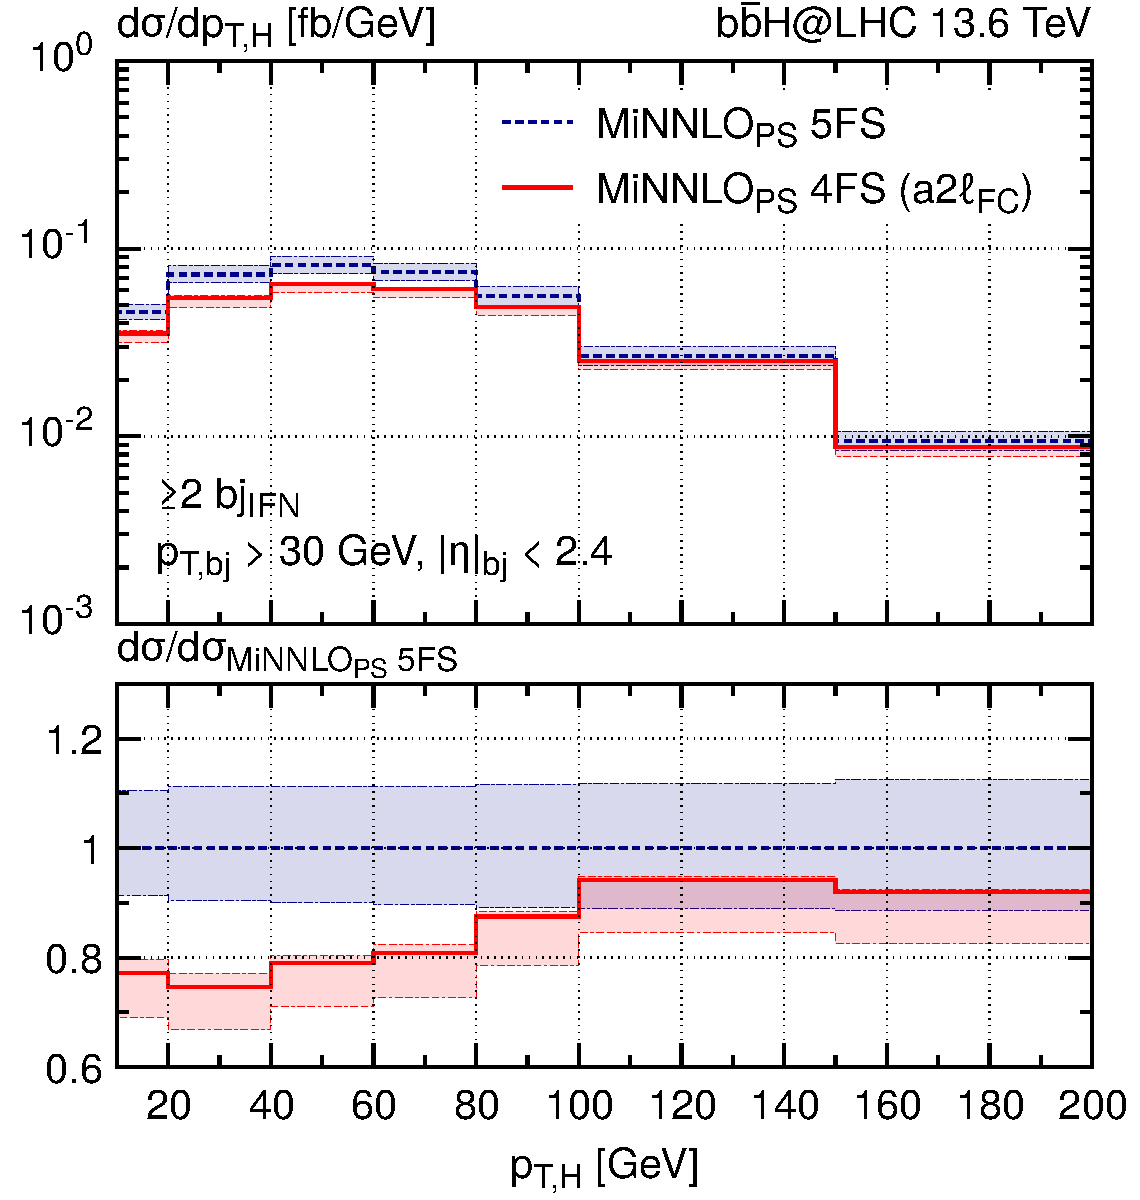
\includegraphics[width=.45\textwidth, page=1]{plots/4fs/pt_H-IFN-2bjet_minnlops-FC.pdf}
\end{tabular}
\vspace*{1ex}
\caption{Higgs transverse momentum spectrum with at least one (left plot) or two (right plot) $b$-jets identified using the IFN algorithm applied to the events generated by \minnlo{} in the massless (blue, dashed) and massive (red, solid) schemes.\label{fig:4fsB}}
\end{center}
\end{figure}

Further insight comes from the Higgs transverse-momentum distribution, shown in figure~\ref{fig:4fsA}. At NLO+PS, the 4FS and 5FS predictions differ significantly at low \(p_{T,H}\). At NNLO+PS, this discrepancy is significantly reduced: \minnlo{} matching brings the two predictions into much better agreement across the full \(p_{T,H}\) range. In particular, in the hard region with \(p_{T,H} \gtrsim 75\)~GeV, the 4FS prediction lies well within the scale uncertainty band of the 5FS prediction.
 
\subsubsection*{Predictions with $b$-jet tagging}
We now turn to the comparison of results with at least one $b$-jet identified in the final state. In this context, the definition of $b$-jets becomes particularly important, especially in the massless 5FS. Applying a jet-flavour algorithm to fixed-order predictions in a massless scheme introduces potential issues due to a mismatch between real and virtual contributions. These mismatches can lead to infrared-unsafe predictions for observables involving flavoured jets, particularly in configurations where a gluon splits into a $b\bar{b}$ pair within the same jet, or when soft, wide-angle $b$-quark emissions are clustered into a jet containing a hard parton. 

%Such divergences arise in tagging strategies like the experimental $b$-tagging definition, referred to as \texttt{EXP} hereafter, which can, however, be directly implemented in the massive 4FS predictions. 
To ensure a theoretically sound and IRC-safe definition of $b$-jets in the massless scheme, we employ the \emph{Interleaved Flavour Neutralisation} (IFN) algorithm~\cite{Caola:2023wpj}, which systematically removes soft $b$-flavour contamination during clustering. In our setup, we use the recommended parameters $\alpha = 2$ and $\omega = 1$. 
%The IFN algorithm is implemented through a dedicated Fortran--C++ interface to the \texttt{FastJet} plugin, allowing seamless integration into our \POWHEG{} framework for all relevant processes.

We now examine the fiducial cross sections in the presence of $b$-jets, comparing 4FS and 5FS predictions at both NLO+PS and NNLO+PS accuracy. As shown in Table~\ref{tab:NNLO4FS_xs}, requiring at least one $b$-jet leads to a significant reduction in the inclusive cross section, by a factor of approximately 5. Imposing a second $b$-jet further suppresses the rate by roughly an additional order of magnitude. These trends are seen across both schemes and perturbative orders. At NNLO+PS, the inclusion of higher-order corrections via \minnlo{} improves the overall consistency between the two schemes, particularly in the one- and two-$b$-jet bins, where 4FS results remain slightly below the 5FS but still agree within uncertainties.

% Interestingly, we observe that the NLO+PS predictions in 4FS and 5FS for the $\geq$2 $b$-jet bin are numerically very close—more so than at NNLO+PS. However, this agreement is accidental. In the 5FS, such observables are less reliable at NLO, since bottom quarks only arise from gluon splittings and are not part of the hard matrix element at Born level. The good agreement at the integrated cross-section level does not reflect the underlying physics accuracy, as will become evident in the following, where we examine the corresponding differential distributions.

Figure~\ref{fig:4fsB} shows the Higgs transverse momentum distribution in events with at least one (left) or two (right) $b$-jets identified using the IFN tagging algorithm. For the inclusive one-$b$-jet selection, the differences between the schemes remain moderate and largely flat. In the two-$b$-jet case, the 4FS prediction is systematically lower than the 5FS, especially in the low and intermediate $p_{T,H}$ regions. This behaviour reflects the more accurate treatment of bottom-quark kinematics in the massive scheme, which becomes particularly relevant when both $b$-jets are required to be hard and well separated.

These results underline the importance of the 4FS computation for observables involving identified $b$-jets. Due to the partonic structure of the 5FS calculation, it lacks accuracy in the hard matrix-element description of $b$-jet production compared to the 4FS. As a result, the 4FS provides a more reliable and accurate prediction, especially in regions sensitive to the kinematics and multiplicity of bottom jets. This makes the 4FS prediction highly relevant for comparisons with experimental measurements involving $b$-tagged final states.
\section{Modelling \bbH{} for background studies in HH searches}
Focus on \citere{Manzoni:2023qaf} mainly (and \citere{Biello:2024pgo}) in fiducial cuts for HH searches (ref. Stefano Manzoni). NNLO+PS ggF generator with different $n_f$ is running using ATLAS resources.
\cbcom{Do not forget to comment bbaa NNLO+PS yb plots.}
\begin{figure}[t!]
\begin{center}
\begin{tabular}{cc}
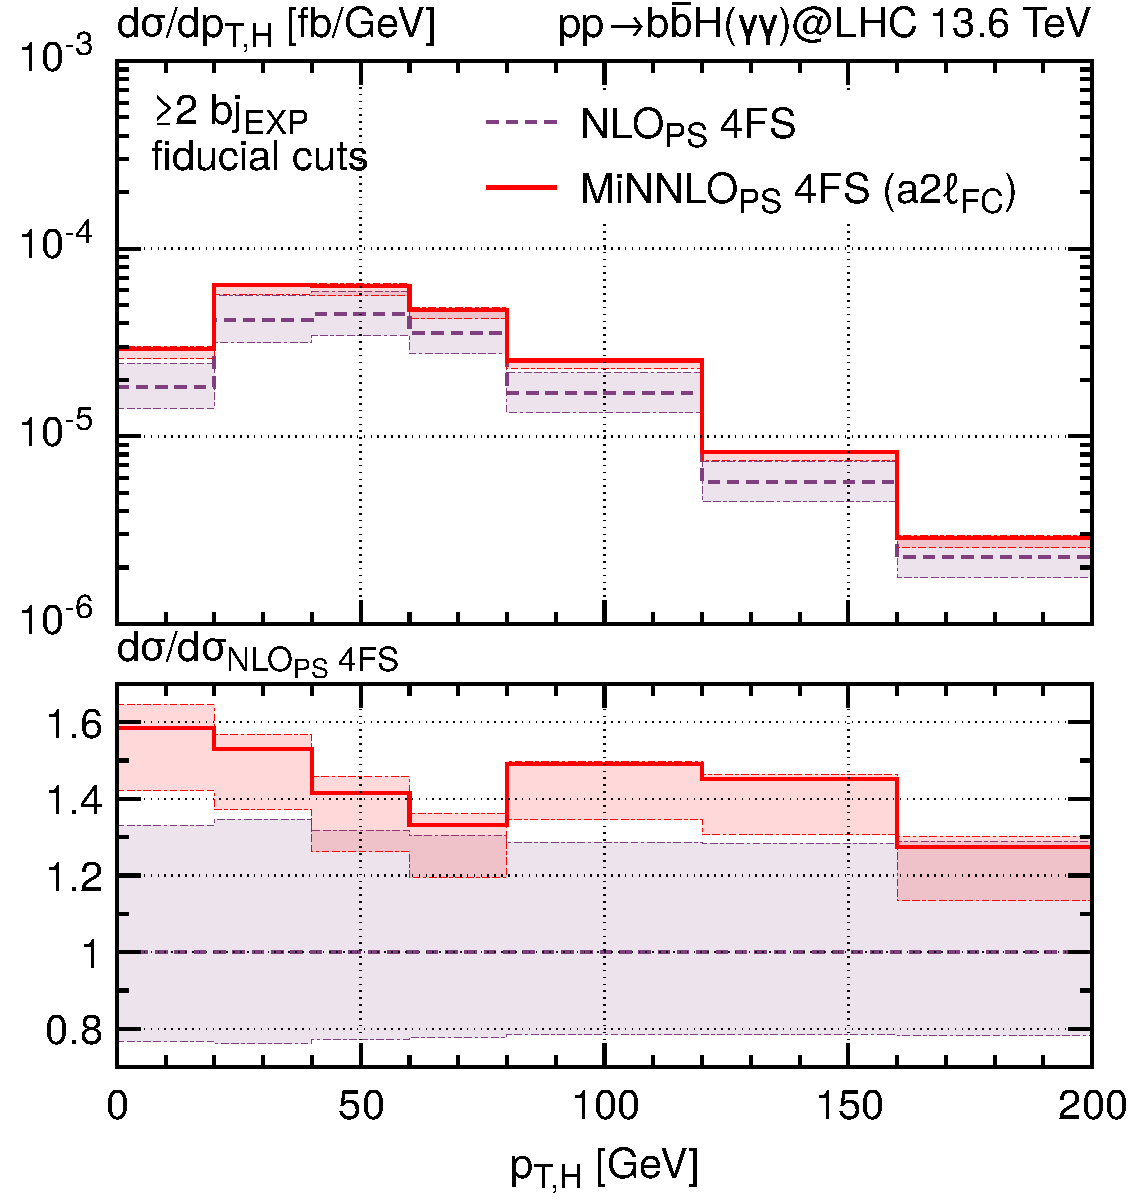
\includegraphics[width=.45\textwidth, page=1]{plots/4fs/pt_Higgs-EXP-fid-FC.pdf}&
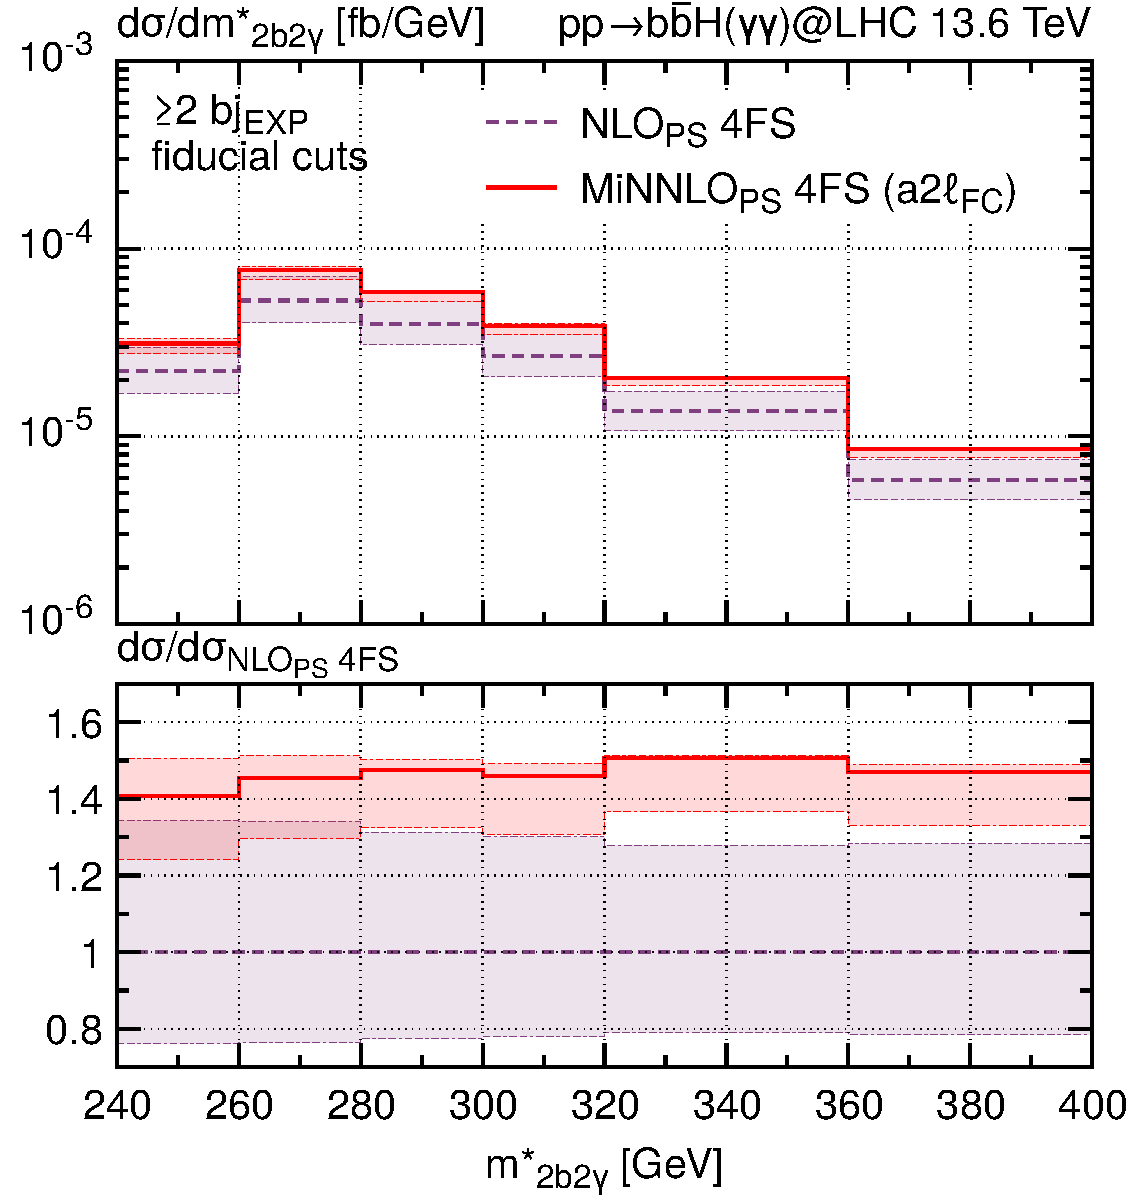
\includegraphics[width=.45\textwidth, page=1]{plots/4fs/mass_2b2gam-EXP-fid-FC.pdf}
\end{tabular}
\vspace*{1ex}
\caption{\label{fig:4fsC}}
\end{center}
\end{figure}

\section{Light-quark Yukawa sensitivity in Higgs spectra}
The \minnlo{} 5FS generator has been recently extended to light-quark parton fusion. These simulations can offer first constraints on anomalously large interactions between the Higgs boson and the light quarks. Indeed, while the bottom-quark Yukawa coupling is strongly constrained through measurements of Higgs decays, no stringent bounds exist for lighter quarks~\cite{Kagan:2014ila}. In particular, the charm Yukawa coupling is only weakly constrained, with an observed upper limit of less than 8.5 times the Standard Model prediction based on analyses of Higgs decay products in Higgsstrahlung events~\cite{Atlas:2022ers}. The development of an NNLO+PS generator for \( q\bar{q} \rightarrow H \) production can provide valuable input for setting constraints on light-quark Yukawa couplings. In particular, it enables the determination of upper bounds for the couplings of up-, down-, and strange-type quarks, owing to the cross-section enhancement driven by their parton distribution functions. 
The cross-section for single Higgs production via parton fusion is given by:
\begin{align}
	\sigma_{\text{H}}(\bar \kappa_q^2)=\sigma_{b\bar b \rightarrow \text{H}}+\bar \kappa_c^2 \bar \sigma_{c\bar c \rightarrow \text{H}}+\bar \kappa_s^2 \bar \sigma_{s\bar s \rightarrow \text{H}}+\bar \kappa_d^2 \bar \sigma_{d\bar d \rightarrow \text{H}}+\bar \kappa_u^2 \bar \sigma_{u\bar u \rightarrow \text{H}}\,.
\end{align}
All interference effects at higher orders vanish due to the massless treatment of the \( n_f = 5 \) parton species. In this context, we introduce the coupling \( \bar\kappa_q \), which denotes the Yukawa coupling of a light quark \( q \), normalised to the Standard-Model Yukawa coupling of the bottom quark in the \MSbar{} scheme. In other words, they represent the cross sections obtained by using \( q \)-flavoured PDFs and assigning the Yukawa interaction the strength of the bottom-quark coupling.

A value of \( \bar\kappa_q = 1 \) corresponds to a Yukawa coupling for quark \( q \) equal in strength to that of the bottom quark. While the SM expectation is \( \kappa_q = 1 \), the normalised couplings take the following values in the SM:  
\( \bar \kappa_u \simeq 5.17 \cdot 10^{-4} \),  
\( \bar \kappa_d \simeq 1.12 \cdot 10^{-3} \),  
\( \bar \kappa_s \simeq 2.2 \cdot 10^{-2} \).
The High-Luminosity Large Hadron Collider prospects~\cite{deBlas:2019rxi} shows that the light-quark Yukawa coupling can be constrained to $|\bar \kappa_u|\leq 0.66$, $|\bar \kappa_d|\leq 0.70$, $|\bar \kappa_s|\leq 0.66$ at 95\% CL when using the transverse momentum distribution.

The simulations are produced using the \minnlo{} \bbH{} generator in the massless scheme as a starting point. The code modifies the flavour of the initial-state partons via the \texttt{whichlightquark} flag, which is set to the Monte Carlo ID number corresponding to the chosen flavour. The generator consistently calls the appropriate analytic amplitudes, with the sole exception of the double real corrections, which are evaluated numerically using the \OpenLoops{} \texttt{bbhjj} library with a suitable flipping of the parton flavours. The number of active massless species is always set to \( n_f = 5 \), including in the running of the strong coupling and Yukawa factors. The theoretical uncertainty is estimated through the standard 7-point scale variation of the factorisation scale for the PDFs and the renormalisation scale with a correlated variation of Yukawa and strong coupling scales.

\subsubsection{Shapes of transverse-momentum spectra}
We begin the phenomenological analysis by focusing on the transverse-momentum spectrum of the Higgs boson. In~\fig{fig:lightpTHzoom}, we show the normalised distribution for the five different flavour channels. By normalising to the total cross section, we remove the dependence on the Yukawa coupling, making the comparison sensitive only to differences in the parton distribution functions (PDFs) across the channels. We observe that the position of the peak varies significantly with the initial-state flavour, with valence-quark channels exhibiting a softer spectrum. The comparatively harder spectrum in the \bbH{} channel is a consequence of the bottom-quark PDF being generated perturbatively, predominantly from gluon splitting.

Although the small masses of the first- and second-generation quarks make their contributions challenging to detect experimentally, the shape of the Higgs transverse-momentum distribution provides a potential handle to disentangle them from the dominant gluon-fusion channel. In particular, the softer spectrum associated with the charm-quark contribution, combined with the intermediate size of its Standard Model Yukawa coupling, makes this observable especially promising for setting experimental constraints in the $c\bar c \text{H}$ mode.

%% If the resummed predictions are available, add in this section

\begin{figure}[t!]
\begin{center}
\begin{tabular}{cc}
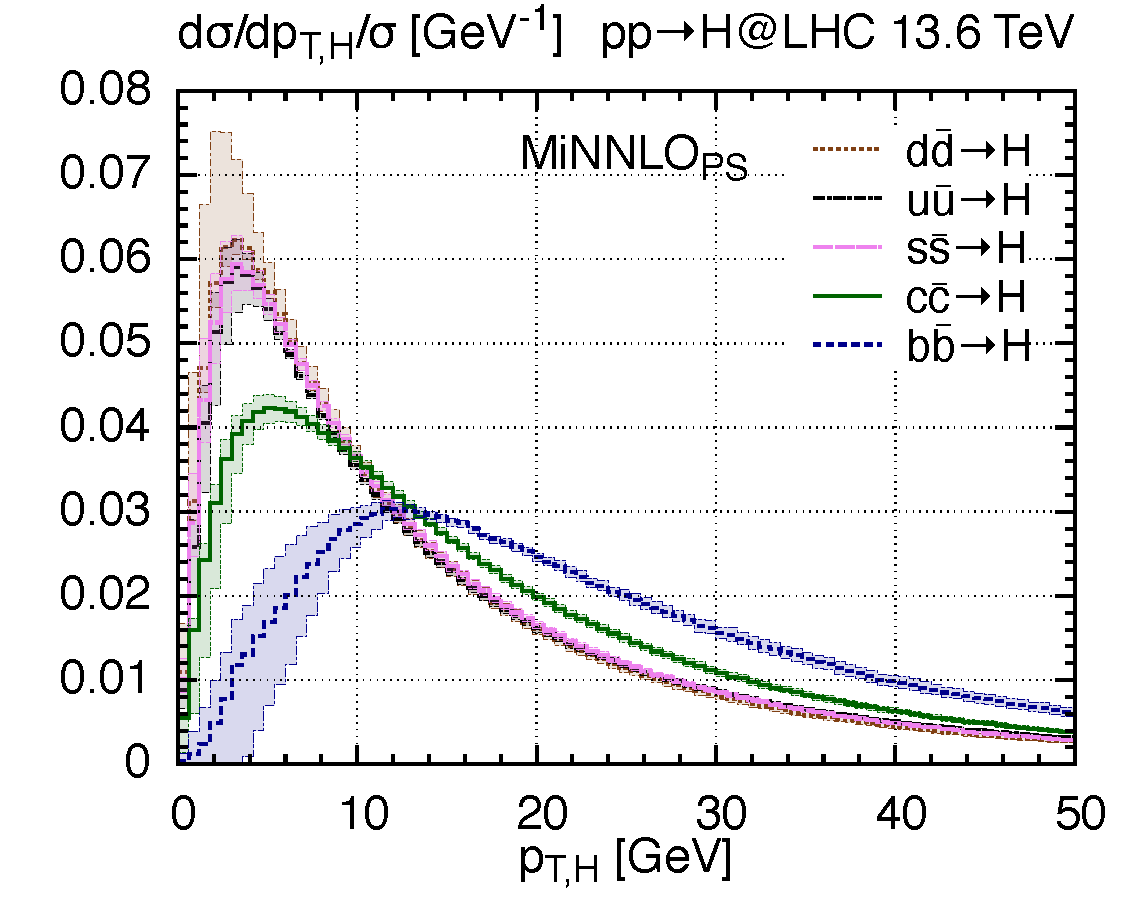
\includegraphics[width=.52\textwidth, page=1]{plots/5fs/light/ptHzoom_qqH.pdf}
\end{tabular}
\vspace*{1ex}
\caption{Transverse-momentum spectra of the Higgs boson obtained with \minnlo{}, normalised to the total cross sections, for the different flavour-channel annihilation: bottom (blue, dashed), charm (green, solid), strange (pink, long-dashed), and down (brown, dotted), and  up (black, dotted-dashed) flavours.
\label{fig:lightpTHzoom}}
\end{center}
\end{figure}

\subsubsection{Simulations with diphoton signature}
In the \POWHEG{} generator, we consider the Higgs boson as an on-shell asymptotic state. We can perform exclusive simulations with colourless decay products by considering the decay into two photons is simulated using the narrow-width approximation in \PYTHIA{8}, assuming a branching fraction of \({\rm BR}(H \to \gamma\gamma) = 0.227\%\)~\cite{LHCHiggsCrossSectionWorkingGroup:2016ypw}. Inspired by a fiducial region accessible by both the ATLAS and CMS detectors we apply the following constraints on the rapidities and transverse momenta of the two photons:
\begin{equation}
|y(\gamma_i)|< 2.37, \quad
\frac{p_T(\gamma_1)}{m(\gamma_1, \gamma_2)} > 0.35,\quad \frac{p_T(\gamma_2)}{m(\gamma_1, \gamma_2)} > 0.25\,. \label{eq:aafidmycuts}
\end{equation}
Here, \( \gamma_1 \) denotes the hardest photon, i.e., the one with the largest transverse momentum. We apply the diphoton \texttt{fiducial cuts} defined in~\eqn{eq:aafidmycuts} and reconstruct the Higgs boson momentum through the components of the photon pair.

To enable cross-checks and comparisons with fixed-order predictions, we have extended the public code \SuSHi{}~\cite{Harlander:2012pb,Harlander:2003ai} to support calculations in light-quark parton fusion. In~\tab{tab:qqH_xs} we present the fully-integrated cross-section values for the total rate of Higgs boson production predicted by the extensions of \SuSHi{} and \minnlo{} according to the setup in~\sct{sec:setup}. We stress that the values are obtained using the bottom-quark Yukawa coupling and must therefore be rescaled by the ratio of the squared quark masses to obtain the correct magnitude of the Standard Model prediction. The central values show an enhancement of the cross section at fixed Yukawa coupling, driven by the parton luminosities. We observe good agreement between the fixed-order and \minnlo{} cross-section predictions, particularly in the down- and up-quark channels. Moreover, the scale uncertainties are significantly reduced in the down, up, and strange channels compared to those involving heavier flavours, most notably the bottom-quark fusion. In the last column of~\tab{tab:qqH_xs} we report the integrated cross-section numbers from the NNLO+PS simulation over the fiducial region defined by the diphoton cuts defined in~\eqn{eq:aafidmycuts}. We stress the different order of magnitude compared to the cross-sections for on-shell Higgs production, due to the Higgs branching ratio into photons. Among the initial-state quarks, the up quark shows the lowest efficiency in passing the fiducial selection, with only about 36\% of diphoton decay events surviving the cuts, compared to approximately 44\% for the down quark and 59\% for the charm quark.
\begin{table}[ht!]
  \vspace*{0.3ex}
  \begin{center}
	   \renewcommand{\arraystretch}{1.3}
    \begin{tabular}{|c||c|c||c|}
    \hline
    \makecell[c]{Flavour channel} & \makecell[c]{\shortstack{$\bar \sigma_{q\bar q \rightarrow \text{H}}$ (pb)\\ \SuSHi{}} } & \makecell[c]{\shortstack{$\bar \sigma_{q\bar q \rightarrow \text{H}}$ (pb)\\ \minnlo{}} }&  \makecell[c]{\shortstack{$\bar \sigma_{q\bar q \rightarrow \text{H}(\rightarrow\gamma \gamma)}$ (fb)\\ \texttt{fiducial $\gamma\gamma$ cuts}\\ \minnlo{}}}  \\
     \hline \hline
	    $d \bar d \rightarrow$ H & $11.46(6)_{-1.1\%}^{+0.5\%}$ & $11.44(2)_{-2.4\%}^{+2.8\%}$ & $11.40(9)_{-2.4\%}^{+2.8\%}$ \\
     \hline
	    $u \bar u \rightarrow$ H & $16.46(6)_{-1.1\%}^{+0.6\%}$ & $16.18(1)_{-2.3\%}^{+2.7\%}$  &  $13.16(9)_{-2.1\%}^{+2.5\%}$ \\
      \hline
	    $s \bar s \rightarrow$ H & $4.45(4)_{-1.4\%}^{+1.0\%}$ & $4.67(6)_{-1.8\%}^{+3.7\%}$  & $6.21(5)_{-1.7\%}^{+3.5\%}$  \\
       \hline
       $c \bar c \rightarrow$ H & $1.84(9)_{-2.9\%}^{+1.5\%}$ & $1.77(8)_{-0.9\%}^{+2.3\%}$  &  $2.40(0)_{-1.0\%}^{+2.3\%}$ \\
        \hline
        $b \bar b \rightarrow$ H &  $0.585(0)_{-9.2\%}^{+7.0\%}$ &  $0.575(7)_{-8.0\%}^{+4.5\%}$ & $0.807(0)_{-8.2\%}^{+4.7\%}$ \\
        \hline
    \end{tabular}
  \end{center}
  \vspace{-1em}
  \caption{
	 Comparison of \SuSHi{} cross-section numbers against the integrated \minnlo{} results for Higgs boson production via light-quark annihilation, with the Yukawa couplings set to the bottom-quark value. The last column presents the NNLO+PS results for $H\rightarrow \gamma\gamma$ production within the fiducial region defined in~\eqn{eq:aafidmycuts}. \label{tab:qqH_xs}}
\end{table}

\begin{figure}[h!]
\begin{center}
\begin{tabular}{cc}
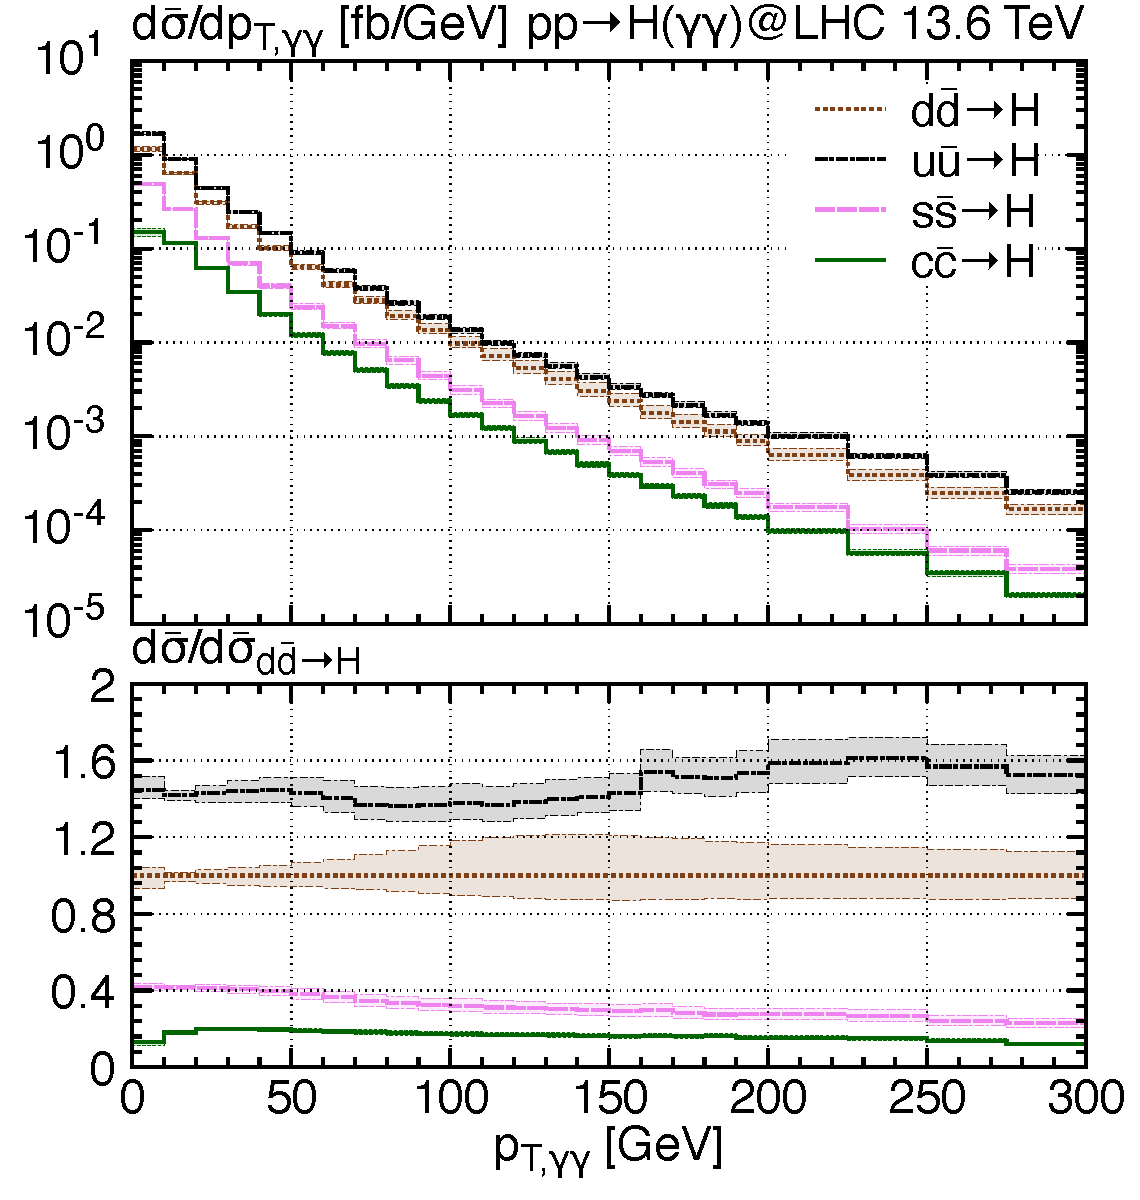
\includegraphics[width=.45\textwidth, page=1]{plots/5fs/light/ptH.pdf}&
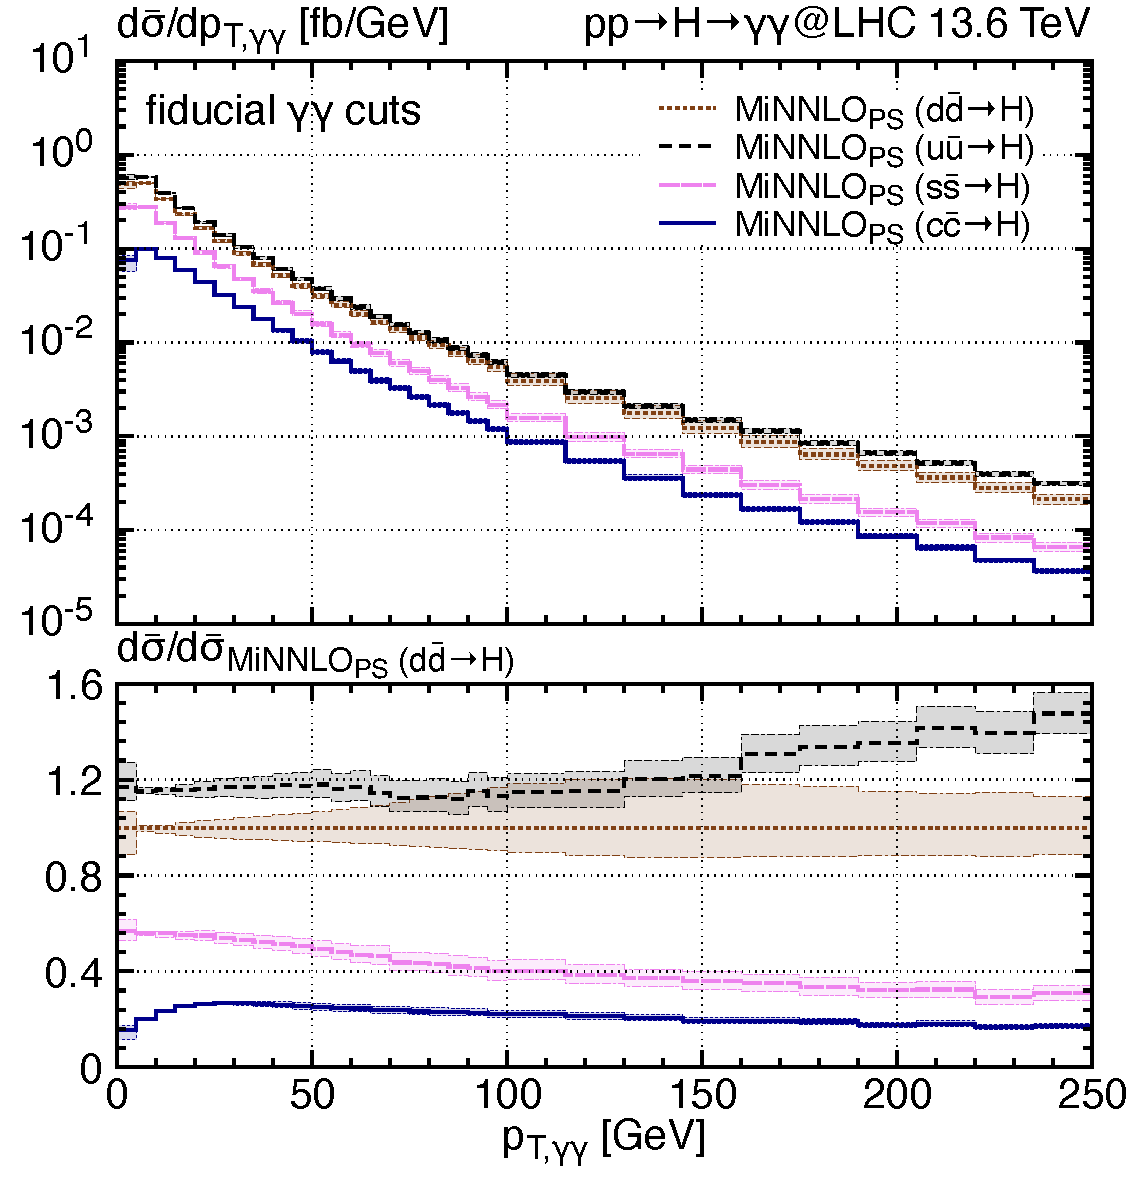
\includegraphics[width=.45\textwidth, page=1]{plots/5fs/light/pt_Higgs-aafid.pdf}
\end{tabular}
\vspace*{1ex}
\caption{Transverse momentum distribution of the reconstructed Higgs boson without cuts (left) and within the fiducial region defined in~\eqn{eq:aafidmycuts} (right).
The results are normalised to the prediction for down-quark fusion (brown, dotted) and compared to those for up- (black, dotted-dashed), strange- (pink, long-dashed), and charm-quark (green, solid) fusion.
\label{fig:lightpTH}}
\end{center}
\end{figure}

\begin{figure}[t!]
\begin{center}
\begin{tabular}{cc}
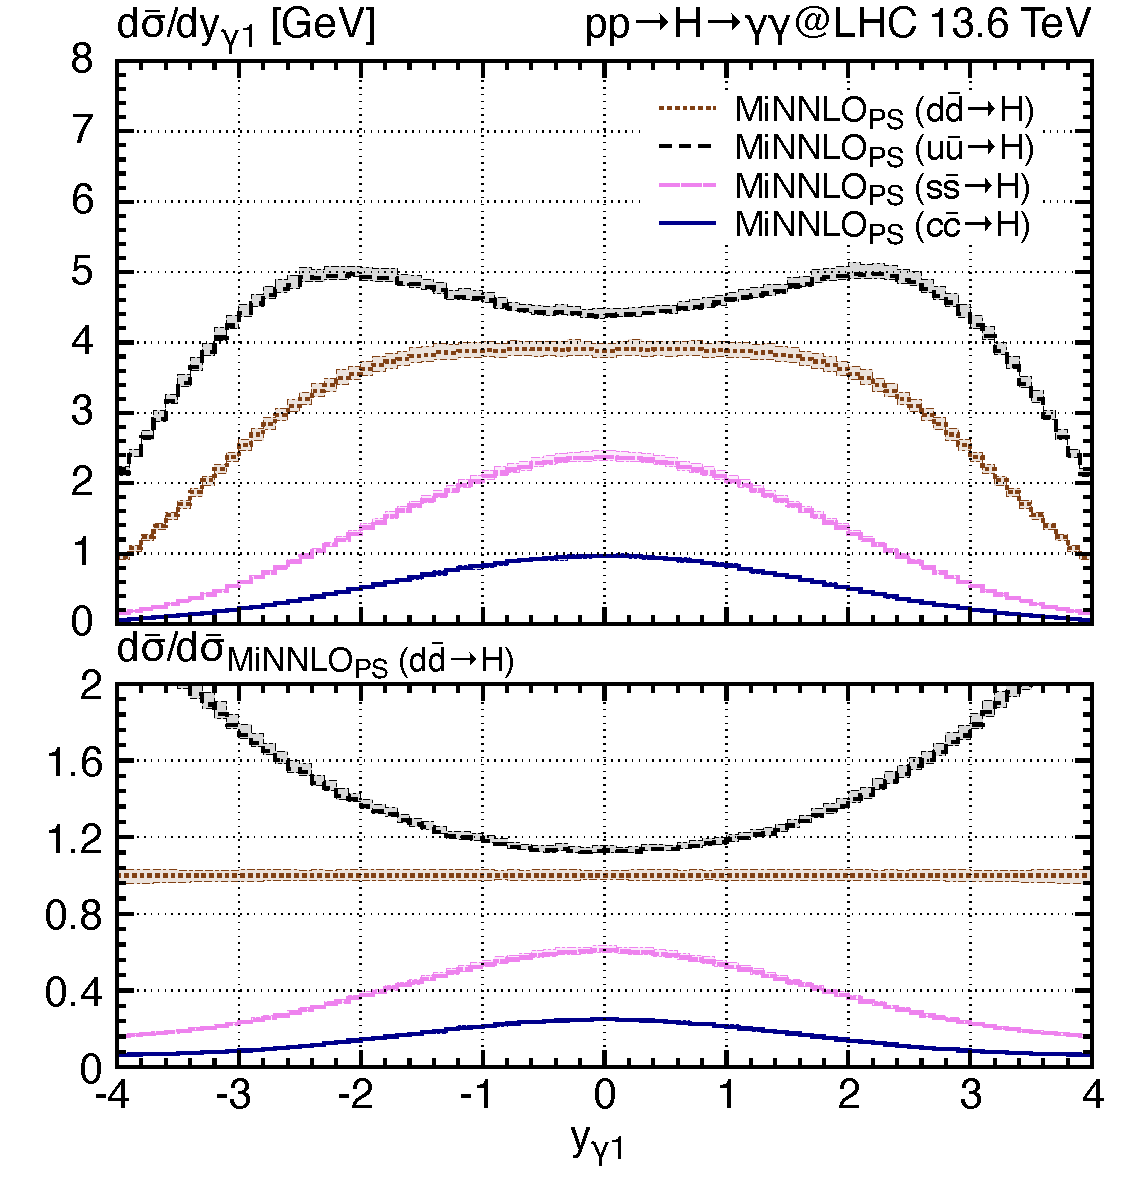
\includegraphics[width=.45\textwidth, page=1]{plots/5fs/light/yphoton1.pdf}&
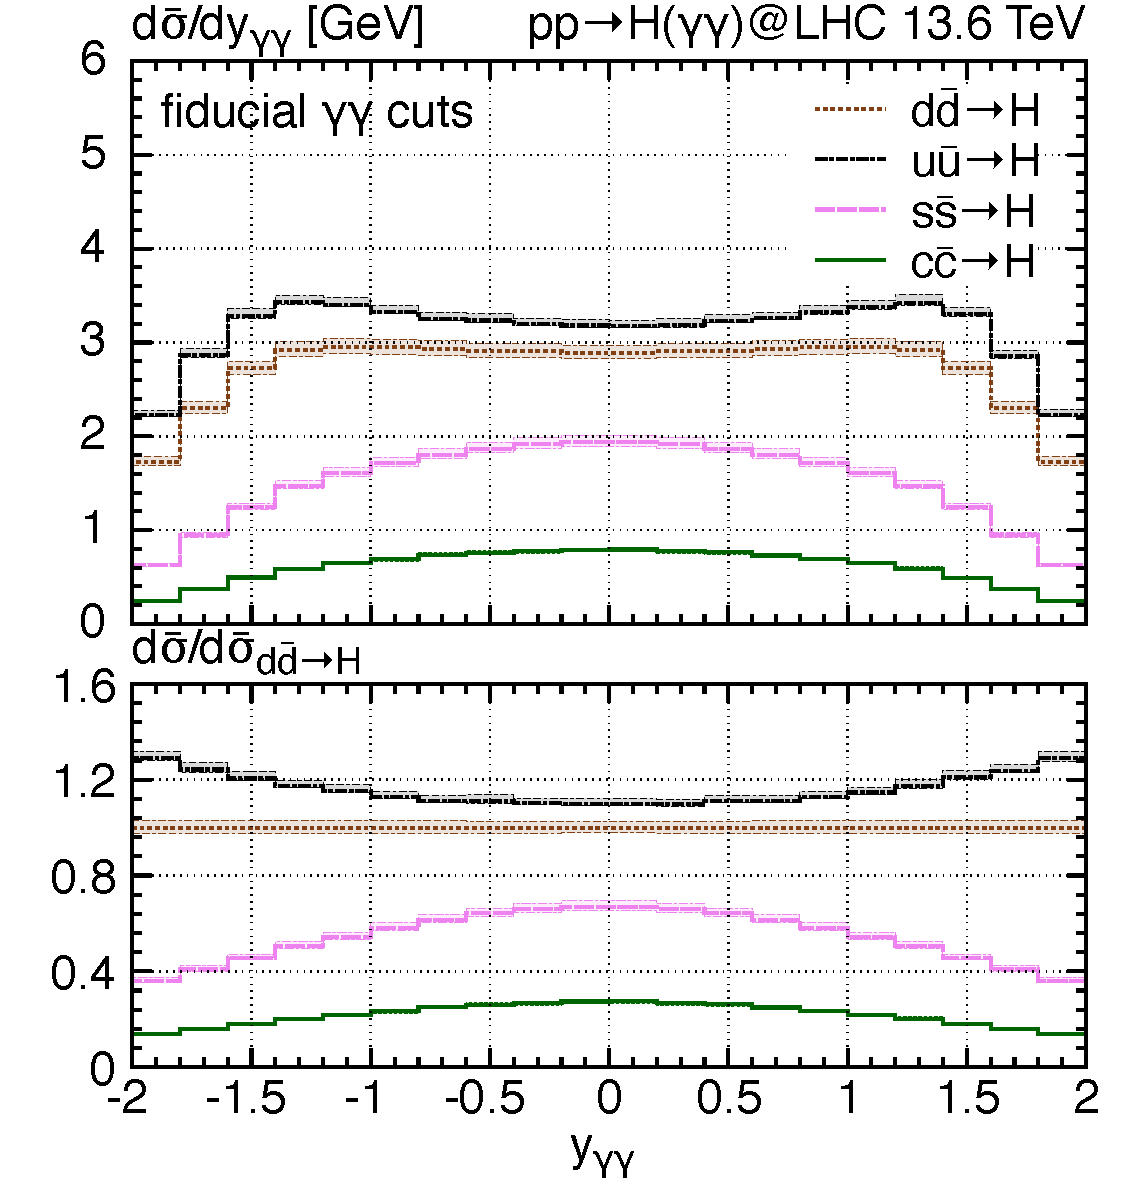
\includegraphics[width=.45\textwidth, page=1]{plots/5fs/light/y_Higgs-aafid.pdf}
\end{tabular}
\vspace*{1ex}
\caption{Rapidity distribution of the hardest photon in the fully inclusive setup (left) and of the reconstructed Higgs boson in the fiducial region (right), for light-parton fusion initiated by up- (black, short-dashed), down- (brown, dotted), strange- (pink, long-dashed), and charm-quarks (blue, solid).\label{fig:lightrapidity}}
\end{center}
\end{figure}

We now present a selection of differential results. The shape of the Higgs transverse momentum spectrum for quark-initiated processes differs significantly from that in the gluon-initiated channel, offering a clearer possibility to study the interaction between the Higgs boson and partons. In the first plot of figure~\ref{fig:lightpTH}, we show the transverse momentum spectrum of the Higgs boson, reconstructed from the diphoton pair in the fully inclusive setup. It displays similar shapes across the different flavour channels, with normalisation reflecting the corresponding total cross sections. The second plot in figure~\ref{fig:lightpTH} shows the same distribution, but for events where the photons pass the fiducial cuts. In this scenario, more pronounced differences in shape emerge among the various channels. In particular, the up-quark contribution—about 1.5 times larger than the down-quark prediction in the fully inclusive case because of PDF enhancement—has a strong reduction in the fiducial region. Indeed, at intermediate values of transverse momentum, the up- and down-quark channels yield comparable results when the same Yukawa strength is assumed. Moreover, once the relative mass suppression in the Yukawa couplings is taken into account, the up-quark prediction falls below the down-quark one.

The main origin of this effect is the rapidity constraint defined in~\eqn{eq:aafidmycuts}. Indeed, the parton distribution functions influence the photon rapidity shape, yielding distinctive behaviour in the up-quark channel. The first plot in figure~\ref{fig:lightrapidity} shows the rapidity distribution of the photon with the highest transverse momentum across the different channels; similar patterns are observed for the second photon. For strange- and charm-quark fusion, as well as for the bottom-quark case, the distribution peaks around zero rapidity. In contrast, valence quark channels exhibit different shapes due to their characteristic parton luminosities. The down-quark channel shows a plateau for $|y_\gamma| < 2$, whereas the up-quark channel features a distribution not centred around zero rapidity, with a significant fraction of the cross section residing at larger rapidity values. As a result, the cut $|y_\gamma| < 2.37$ has a more pronounced impact on the up-quark distribution, removing a larger portion of the cross section when applying the fiducial selection. We have confirmed a similar trend at leading order, with a shape validated using the mass-rapidity scan of PDF4LHC luminosities obtained using \texttt{APFEL}~\cite{Bertone:2013vaa}. This distinctive behaviour, more evident here than in neutral Drell–Yan due to the higher Higgs mass, provides a useful handle for differential studies, as the rapidity spectrum in light-quark fusion differs markedly from dominant production modes. We conclude by presenting the Higgs boson rapidity, reconstructed from the two photons that satisfy the fiducial cuts~\eqref{eq:aafidmycuts}, as shown in the second plot of figure~\ref{fig:lightrapidity}. In the exclusive region, the up-quark behaviour is more similar to the down-quark, with a cross section between 1.1 and 1.3 times that of the down-quark process. The charm-quark and the strange-quark exhibit a steeper distribution compared to the Higgs boson from down-quark fusion.

In this section, we have presented the NNLO+PS generator for Higgs production via light-parton fusion with decay into photons as a potential tool to constrain light-quark Yukawa couplings. We conclude by noting that alternative channels sensitive to light-quark Yukawa couplings have been experimentally investigated recently, such as the Higgs decay rate into four leptons~\cite{CMS:2025xkn}.
\section{Outlooks and Conclusions}
Conclusions.\\
\cbcom{Outlooks: ccH in 3FS at NNLO+PS, alternative estimation of HH background in yt, flavour-matched predictions at differential level with Rhorry or sACOT}

\textbf{Citation policy. }The present work consists of contributions from different collaborations. If some of the results are employed for scientific publications, together with this work, one should cite the corresponding work in~\citeres{Manzoni:2023qaf,Cal:2023mib,Biello:2024vdh,Biello:2024pgo,Gavardi:2025zpf}.

\textbf{Acknowledgements. }This work has been carried out within the LHC Higgs Working Group, as a contribution to the Yellow Report 5. We thank all the WG3 conveners for coordinating the activities, in particular Tatjana Lenz. CB is grateful to Tommaso Giani for PDF insights and Jan Lukas Spah for interesting discussions on Yukawa interactions via light-quark fusion. We have used the Max Planck Computing and Data Facility (MPCDF) in Garching to carry out the \minnlo{} simulations presented here for \bbtoH{}, $q\bar q\rightarrow \text{H}$ and \bbH{} production.

\bibliography{bbh}
\bibliographystyle{JHEP}

\end{document}
